% Generated by Sphinx.
\documentclass[letterpaper,10pt,english]{manual}
\usepackage[utf8]{inputenc}
\usepackage[T1]{fontenc}
\usepackage{babel}
\usepackage{times}
\usepackage[Bjarne]{fncychap}
\usepackage{sphinx}
\usepackage{amssymb}

\title{Sage Sandpiles Documentation}
\date{December 25, 2009}
\release{2.0}
\author{David Perkinson}
\newcommand{\sphinxlogo}{}
\renewcommand{\releasename}{Release}
\makeindex
\makemodindex

\makeatletter
\def\PYG@reset{\let\PYG@it=\relax \let\PYG@bf=\relax%
    \let\PYG@ul=\relax \let\PYG@tc=\relax%
    \let\PYG@bc=\relax \let\PYG@ff=\relax}
\def\PYG@tok#1{\csname PYG@tok@#1\endcsname}
\def\PYG@toks#1+{\ifx\relax#1\empty\else%
    \PYG@tok{#1}\expandafter\PYG@toks\fi}
\def\PYG@do#1{\PYG@bc{\PYG@tc{\PYG@ul{%
    \PYG@it{\PYG@bf{\PYG@ff{#1}}}}}}}
\def\PYG#1#2{\PYG@reset\PYG@toks#1+\relax+\PYG@do{#2}}

\def\PYG@tok@gu{\let\PYG@bf=\textbf\def\PYG@tc##1{\textcolor[rgb]{0.50,0.00,0.50}{##1}}}
\def\PYG@tok@gt{\def\PYG@tc##1{\textcolor[rgb]{0.00,0.25,0.82}{##1}}}
\def\PYG@tok@gs{\let\PYG@bf=\textbf}
\def\PYG@tok@gr{\def\PYG@tc##1{\textcolor[rgb]{1.00,0.00,0.00}{##1}}}
\def\PYG@tok@cm{\let\PYG@it=\textit\def\PYG@tc##1{\textcolor[rgb]{0.25,0.50,0.56}{##1}}}
\def\PYG@tok@vg{\def\PYG@tc##1{\textcolor[rgb]{0.73,0.38,0.84}{##1}}}
\def\PYG@tok@m{\def\PYG@tc##1{\textcolor[rgb]{0.13,0.50,0.31}{##1}}}
\def\PYG@tok@mh{\def\PYG@tc##1{\textcolor[rgb]{0.13,0.50,0.31}{##1}}}
\def\PYG@tok@go{\def\PYG@tc##1{\textcolor[rgb]{0.19,0.19,0.19}{##1}}}
\def\PYG@tok@ge{\let\PYG@it=\textit}
\def\PYG@tok@gd{\def\PYG@tc##1{\textcolor[rgb]{0.63,0.00,0.00}{##1}}}
\def\PYG@tok@il{\def\PYG@tc##1{\textcolor[rgb]{0.13,0.50,0.31}{##1}}}
\def\PYG@tok@cs{\def\PYG@tc##1{\textcolor[rgb]{0.25,0.50,0.56}{##1}}\def\PYG@bc##1{\colorbox[rgb]{1.00,0.94,0.94}{##1}}}
\def\PYG@tok@cp{\def\PYG@tc##1{\textcolor[rgb]{0.00,0.44,0.13}{##1}}}
\def\PYG@tok@gi{\def\PYG@tc##1{\textcolor[rgb]{0.00,0.63,0.00}{##1}}}
\def\PYG@tok@gh{\let\PYG@bf=\textbf\def\PYG@tc##1{\textcolor[rgb]{0.00,0.00,0.50}{##1}}}
\def\PYG@tok@ni{\let\PYG@bf=\textbf\def\PYG@tc##1{\textcolor[rgb]{0.84,0.33,0.22}{##1}}}
\def\PYG@tok@nl{\let\PYG@bf=\textbf\def\PYG@tc##1{\textcolor[rgb]{0.00,0.13,0.44}{##1}}}
\def\PYG@tok@nn{\let\PYG@bf=\textbf\def\PYG@tc##1{\textcolor[rgb]{0.05,0.52,0.71}{##1}}}
\def\PYG@tok@no{\def\PYG@tc##1{\textcolor[rgb]{0.38,0.68,0.84}{##1}}}
\def\PYG@tok@na{\def\PYG@tc##1{\textcolor[rgb]{0.25,0.44,0.63}{##1}}}
\def\PYG@tok@nb{\def\PYG@tc##1{\textcolor[rgb]{0.00,0.44,0.13}{##1}}}
\def\PYG@tok@nc{\let\PYG@bf=\textbf\def\PYG@tc##1{\textcolor[rgb]{0.05,0.52,0.71}{##1}}}
\def\PYG@tok@nd{\let\PYG@bf=\textbf\def\PYG@tc##1{\textcolor[rgb]{0.33,0.33,0.33}{##1}}}
\def\PYG@tok@ne{\def\PYG@tc##1{\textcolor[rgb]{0.00,0.44,0.13}{##1}}}
\def\PYG@tok@nf{\def\PYG@tc##1{\textcolor[rgb]{0.02,0.16,0.49}{##1}}}
\def\PYG@tok@si{\let\PYG@it=\textit\def\PYG@tc##1{\textcolor[rgb]{0.44,0.63,0.82}{##1}}}
\def\PYG@tok@s2{\def\PYG@tc##1{\textcolor[rgb]{0.25,0.44,0.63}{##1}}}
\def\PYG@tok@vi{\def\PYG@tc##1{\textcolor[rgb]{0.73,0.38,0.84}{##1}}}
\def\PYG@tok@nt{\let\PYG@bf=\textbf\def\PYG@tc##1{\textcolor[rgb]{0.02,0.16,0.45}{##1}}}
\def\PYG@tok@nv{\def\PYG@tc##1{\textcolor[rgb]{0.73,0.38,0.84}{##1}}}
\def\PYG@tok@s1{\def\PYG@tc##1{\textcolor[rgb]{0.25,0.44,0.63}{##1}}}
\def\PYG@tok@vc{\def\PYG@tc##1{\textcolor[rgb]{0.73,0.38,0.84}{##1}}}
\def\PYG@tok@sh{\def\PYG@tc##1{\textcolor[rgb]{0.25,0.44,0.63}{##1}}}
\def\PYG@tok@ow{\let\PYG@bf=\textbf\def\PYG@tc##1{\textcolor[rgb]{0.00,0.44,0.13}{##1}}}
\def\PYG@tok@mf{\def\PYG@tc##1{\textcolor[rgb]{0.13,0.50,0.31}{##1}}}
\def\PYG@tok@bp{\def\PYG@tc##1{\textcolor[rgb]{0.00,0.44,0.13}{##1}}}
\def\PYG@tok@c1{\let\PYG@it=\textit\def\PYG@tc##1{\textcolor[rgb]{0.25,0.50,0.56}{##1}}}
\def\PYG@tok@kc{\let\PYG@bf=\textbf\def\PYG@tc##1{\textcolor[rgb]{0.00,0.44,0.13}{##1}}}
\def\PYG@tok@c{\let\PYG@it=\textit\def\PYG@tc##1{\textcolor[rgb]{0.25,0.50,0.56}{##1}}}
\def\PYG@tok@sx{\def\PYG@tc##1{\textcolor[rgb]{0.78,0.36,0.04}{##1}}}
\def\PYG@tok@err{\def\PYG@bc##1{\fcolorbox[rgb]{1.00,0.00,0.00}{1,1,1}{##1}}}
\def\PYG@tok@kd{\let\PYG@bf=\textbf\def\PYG@tc##1{\textcolor[rgb]{0.00,0.44,0.13}{##1}}}
\def\PYG@tok@ss{\def\PYG@tc##1{\textcolor[rgb]{0.32,0.47,0.09}{##1}}}
\def\PYG@tok@sr{\def\PYG@tc##1{\textcolor[rgb]{0.14,0.33,0.53}{##1}}}
\def\PYG@tok@mo{\def\PYG@tc##1{\textcolor[rgb]{0.13,0.50,0.31}{##1}}}
\def\PYG@tok@kn{\let\PYG@bf=\textbf\def\PYG@tc##1{\textcolor[rgb]{0.00,0.44,0.13}{##1}}}
\def\PYG@tok@mi{\def\PYG@tc##1{\textcolor[rgb]{0.13,0.50,0.31}{##1}}}
\def\PYG@tok@gp{\let\PYG@bf=\textbf\def\PYG@tc##1{\textcolor[rgb]{0.78,0.36,0.04}{##1}}}
\def\PYG@tok@o{\def\PYG@tc##1{\textcolor[rgb]{0.40,0.40,0.40}{##1}}}
\def\PYG@tok@kr{\let\PYG@bf=\textbf\def\PYG@tc##1{\textcolor[rgb]{0.00,0.44,0.13}{##1}}}
\def\PYG@tok@s{\def\PYG@tc##1{\textcolor[rgb]{0.25,0.44,0.63}{##1}}}
\def\PYG@tok@kp{\def\PYG@tc##1{\textcolor[rgb]{0.00,0.44,0.13}{##1}}}
\def\PYG@tok@w{\def\PYG@tc##1{\textcolor[rgb]{0.73,0.73,0.73}{##1}}}
\def\PYG@tok@kt{\def\PYG@tc##1{\textcolor[rgb]{0.56,0.13,0.00}{##1}}}
\def\PYG@tok@sc{\def\PYG@tc##1{\textcolor[rgb]{0.25,0.44,0.63}{##1}}}
\def\PYG@tok@sb{\def\PYG@tc##1{\textcolor[rgb]{0.25,0.44,0.63}{##1}}}
\def\PYG@tok@k{\let\PYG@bf=\textbf\def\PYG@tc##1{\textcolor[rgb]{0.00,0.44,0.13}{##1}}}
\def\PYG@tok@se{\let\PYG@bf=\textbf\def\PYG@tc##1{\textcolor[rgb]{0.25,0.44,0.63}{##1}}}
\def\PYG@tok@sd{\let\PYG@it=\textit\def\PYG@tc##1{\textcolor[rgb]{0.25,0.44,0.63}{##1}}}

\def\PYGZat{@}
\def\PYGZlb{[}
\def\PYGZrb{]}
\makeatother

\begin{document}

\maketitle
\tableofcontents




\chapter{Introduction}

Sage Sandpiles is a package for calculations involving Dhar's abelian sandpile
model (ASM) using the open-source mathematics software, Sage.  A brief
introduction to the ASM follows.  For a more thorough introduction, the papers
\emph{Chip-Firing and Rotor-Routing on Directed Graphs} {[}H{]}, by Holroyd et al. and
\emph{Riemann-Roch and Abel-Jacobi Theory on a Finite Graph} by Baker and Norine
{[}BN{]} are recommended.

To describe the ASM, we start with a \emph{sandpile graph}: a directed multigraph
$\Gamma$ with a vertex $s$ that is accessible from every vertex (except
possible $s$, itself).  By \emph{multigraph}, we mean that each edge of $\Gamma$ is
assigned a nonnegative integer weight.  To say $s$ is \emph{accessible} from some
vertex $v$ means that there is a sequence of directed edges starting at $v$ and
ending at $s$.  We call $s$ the \emph{sink} of the sandpile graph, even though it might have outgoing edges, for reasons that will be made clear in a moment.

We denoted the vertices of $\Gamma$ by $V$ and define $\tilde{V} = V\setminus\{s\}$.


\section{Configurations and divisors}

A \emph{configuration} on $\Gamma$ is an element of $\mathbb{N}\tilde{V}$, i.e., the
assignment of a nonnegative integer to each nonsink vertex.  We think of each
integer as a number of grains of sand being placed at the corresponding
vertex.  A \emph{divisor} on $\Gamma$ is an element of $\mathbb{Z}V$, i.e., an
element in the free abelian group on \emph{all} of the vertices.  In the context of
divisors, it is sometimes useful to think of assigning dollars to each vertex,
with negative integers signifying a debt.


\section{Stabilization}

A configuration $c$ is \emph{stable} at a vertex $v\in\tilde{V}$ if
$c(v)<\mbox{out-degree}(v)$, and $c$ itself is stable if it is stable at each
nonsink vertex.  If $c$ is unstable at $v$, the vertex $v$ can be \emph{fired}
(\emph{toppled}) by removing $\mbox{out-degree}(v)$ grains of sand from $v$ and
adding grains of sand to the neighbors of sand, determined by the weights of
the edges leaving $v$.

Despite our best intentions, we sometimes consider firing a stable vertex,
resulting in a configuration with a ``negative amount'' of sand at that vertex.
We may also \emph{reverse-firing} a vertex, absorbing sand from the vertex's
neighbors.

\textbf{Example.} Consider the graph:
\begin{figure}[htbp]
\centering

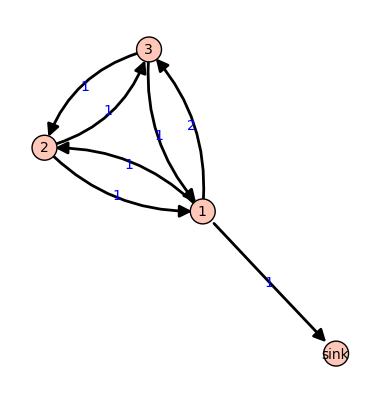
\includegraphics{example1.png}
\caption{$\Gamma$}\end{figure}

All edges have weight $1$ except for the edge from vertex 1 to vertex 3,
which have weight $2$.  If we let $c=(5,0,1)$ with the indicated number of
grains of sand on vertices 1, 2, and 3, respectively, then only vertex 1,
whose out-degree is 4, is unstable.  Firing vertex 1 gives a new
configuration $c'=(1,1,3)$.  Here, $4$ grains have left vertex 1.  One of
these has gone to the sink vertex (and forgotten), one has gone to vertex 1,
and two have gone to vertex 2, since the edge from 1 to 2 has weight 2.
Vertex 3 in the new configuration is now unstable.  The Sage code for this
example looks like this:

\begin{Verbatim}[commandchars=@\[\]]
Create the sandpile:

    sage: load sandpile.sage
    sage: g = {'sink':{},
               1:{'sink':1, 2:1, 3:2},
               2:{1:1, 3:1},
               3:{1:1, 2:1}}
    sage: S = Sandpile(g, 'sink')
    sage: S.show(edge@_labels=true)  @# to display the graph

Create the configuration:

    sage: c = Config(S, {1:5, 2:0, 3:1})
    sage: S.out@_degree()
    {1: 4, 2: 2, 3: 2, 'sink': 0}

Fire vertex one:

   sage: c.fire@_vertex(1,c)
   {1: 1, 2: 1, 3: 3}

The configuration is unchanged:

    sage: c
    {1: 5, 2: 0, 3: 1}

Repeatedly fire vertices until the configuration becomes stable:

    sage: c.stabilize()
    {1: 2, 2: 1, 3: 1}

Alternatives:

    sage: @textasciitilde[]c             @# shorthand for c.stabilize()
    {1: 2, 2: 1, 3: 1}
    sage: c.stabilize(with@_firing@_vector=true)
    @PYGZlb[]{1: 2, 2: 1, 3: 1}, {1: 2, 2: 2, 3: 3}@PYGZrb[]
\end{Verbatim}

Since vertex 3 has become unstable after firing vertex 1, it can be fired,
which causes vertex 2 to become unstable, etc.  Repeated firings eventually
lead to a stable configuration.  The last line of the Sage code, above, is a
list, the first element of which is the resulting stable configuration,
$(2,1,1)$.  The second component records how many times each vertex fired in
the stabilization.


\bigskip\hrule{}\bigskip


Since the sink is accessible from each nonsink vertex and never fires, every
configuration will stabilize after a finite number of vertex-firings.  It is
not obvious, but the resulting stabilization is independent of the order in
which unstable vertices are fired.  Thus, each configuration stabilizes to a
unique stable configuration.


\section{Laplacian}

Fix an order on the vertices of $\Gamma$. The \emph{Laplacian} of $\Gamma$ is
\begin{gather}
\begin{split}L := D-A\end{split}\notag
\end{gather}
where $D$ is the diagonal matrix of out-degrees of the vertices and $A$ is the
adjacency matrix whose $(i,j)$-th entry is the weight of the edge from vertex
$i$ to vertex $j$, which we take to be $0$ if there is no edge.  The \emph{reduced
Laplacian}, $\tilde{L}$, is the submatrix of the Laplacian formed by removing
the row and column corresponding to the sink vertex.  Firing a vertex of a
configuration is the same as subtracting the corresponding row of the reduced
Laplacian.

\textbf{Example.} (Continued.)

\begin{Verbatim}[commandchars=@\[\]]
    sage: S.vertices()  @# here is the ordering of the vertices
    @PYGZlb[]1, 2, 3, 'sink'@PYGZrb[]
    sage: S.laplacian()
    @PYGZlb[] 4 -1 -2 -1@PYGZrb[]
    @PYGZlb[]-1  2 -1  0@PYGZrb[]
    @PYGZlb[]-1 -1  2  0@PYGZrb[]
    @PYGZlb[] 0  0  0  0@PYGZrb[]
    sage: S.reduced@_laplacian()
    @PYGZlb[] 4 -1 -2@PYGZrb[]
    @PYGZlb[]-1  2 -1@PYGZrb[]
    @PYGZlb[]-1 -1  2@PYGZrb[]

The configuration we considered previously:

    sage: c = Config(S, @PYGZlb[]5,0,1@PYGZrb[])
    sage: c
    {1: 5, 2: 0, 3: 1}

Firing vertex 1 is the same as subtracting the
corresponding row from the reduced Laplacian:

    sage: c.fire@_vertex(1).values()
    @PYGZlb[]1, 1, 3@PYGZrb[]
    sage: S.reduced@_laplacian()@PYGZlb[]0@PYGZrb[]
    (4, -1, -2)
    sage: vector(@PYGZlb[]5,0,1@PYGZrb[]) - vector(@PYGZlb[]4,-1,-2@PYGZrb[])
    (1, 1, 3)
\end{Verbatim}


\section{Recurrent elements}

Imagine an experiment in which grains of sand are dropped one-at-a-time onto a
graph, pausing to allow the configuration to stabilize between drops.  Some
configurations will only be seen once in this process.  For example, for most
graphs, once sand is dropped on the graph, no addition of sand+stabilization
will result in a graph empty of sand.  Other configurations---the so-called
\emph{recurrent configurations}---will be seen infinitely often as the process is
repeated indefinitely.

To be precise, a configuration $c$ is \emph{recurrent} if (i) it is stable, and (ii)
given any configuration $a$, there is a configuration $b$ such that
$c=\mbox{stab}(a+b)$, the stabilization of $a+b$.

The \emph{maximal-stable} configuration, denoted $c_{\mathrm{max}}$ is defined by
$c_{\mathrm{max}}(v)=\mbox{out-degree}(v)-1$ for all nonsink vertices $v$.  It is clear that $c_{\mathrm{max}}$ is recurrent.  Further, it is not hard to see that a configuration is recurrent if and only if it has the form $\mbox{stab}(a+c_{\mathrm{max}})$ for some configuration $a$.

\textbf{Example.} (Continued.)

\begin{Verbatim}[commandchars=@\[\]]
    sage: S.recurrents(verbose=false)
    @PYGZlb[]@PYGZlb[]3, 1, 1@PYGZrb[], @PYGZlb[]2, 1, 1@PYGZrb[], @PYGZlb[]3, 1, 0@PYGZrb[]@PYGZrb[]
    sage: c = Config(S, @PYGZlb[]2,1,1@PYGZrb[])
    sage: c
    {1: 2, 2: 1, 3: 1}
    sage: S.is@_recurrent(c)
    True
    sage: S.max@_stable()
    {1: 3, 2: 1, 3: 1}

Adding any configuration to the max-stable configuration and stabilizing
yields a recurrent configuration.

    sage: x = Config(S, @PYGZlb[]1,0,0@PYGZrb[])
    sage: x + S.max@_stable()
    {1: 4, 2: 1, 3: 1}

Use @& to add and stabilize:

    sage: c = x @& S.max@_stable()
    sage: c
    {1: 3, 2: 1, 3: 0}
    sage: c.is@_recurrent()
    True

Note the various ways of performing addition + stabilization:

    sage: (x + m).stabilize() == @textasciitilde[](x + m)
    True
    sage: (x + m).stabilize() == x @& m
    True
\end{Verbatim}


\section{Burning Configuration}

A \emph{burning configuration} is a nonnegative integer-linear combination of the
rows of the reduced Laplacian matrix having nonnegative entries and such that
every vertex has a path from some vertex in its support.  The corresponding
\emph{burning script} gives the integer-linear combination needed to obtain the
burning configuration.  So if $b$ is the burning configuration, $\sigma$ is its
script, and $\tilde{L}$ is the reduced Laplacian, then $\sigma\,\tilde{L} = b$.
The \emph{minimal burning configuration} is the one with the minimal script (its
components are no larger than the components of any other script for a burning
configuration).

The following are equivalent for a configuration $c$ with burning
configuration $b$ having script $\sigma$:
\begin{itemize}
\item {} 
$c$ is recurrent;

\item {} 
$c+b$ stabilizes to $c$;

\item {} 
the firing vector for the stabilization of $c+b$ is $\sigma$.

\end{itemize}

The burning configuration and script are computed using a modified
version of Speer's script algorithm.  This is a generalization to
directed multigraphs of Dhar's burning algorithm.

\textbf{Example.}

\begin{Verbatim}[commandchars=@\[\]]
sage: g = {0:{},1:{0:1,3:1,4:1},2:{0:1,3:1,5:1},
           3:{2:1,5:1},4:{1:1,3:1},5:{2:1,3:1}}
sage: G = Sandpile(g,0)
sage: G.burning@_config()
{1: 2, 2: 0, 3: 1, 4: 1, 5: 0}
sage: G.burning@_config().values()
@PYGZlb[]2, 0, 1, 1, 0@PYGZrb[]
sage: G.burning@_script()
{1: 1, 2: 3, 3: 5, 4: 1, 5: 4}
sage: G.burning@_script().values()
@PYGZlb[]1, 3, 5, 1, 4@PYGZrb[]
sage: matrix(G.burning@_script().values())*G.reduced@_laplacian()
@PYGZlb[]2 0 1 1 0@PYGZrb[]
\end{Verbatim}


\section{Sandpile group}

The collection of stable configurations forms a commutative monoid with
addition defined as ordinary addition followed by stabilization.  The identity
element is the all-zero configuration.  This monoid is a group
exactly when the underlying graph is a DAG (directed acyclic graph).

The recurrent elements form a submonoid which turns out to be a group.  This
group is called the \emph{sandpile group} for $\Gamma$, denoted
$\mathcal{S}(\Gamma)$.  Its identity element is usually not the all-zero
configuration (again, only in the case that $\Gamma$ is a DAG).  So finding the
identity element is an interesting problem.

Let $n=|V|-1$ and fix an ordering of the nonsink vertices. Let
$\mathcal{\tilde{L}}\subset\mathbb{Z}^n$ denote the column-span of
$\tilde{L}^t$, the transpose of the reduced Laplacian.  It is a theorem that
\begin{gather}
\begin{split}\mathcal{S}(\Gamma)\approx \mathbb{Z}^n/\mathcal{\tilde{L}}.\end{split}\notag
\end{gather}
Thus, the number of elements of the sandpile group is $\det{\tilde{L}}$, which
by the matrix-tree theorem is the number of weighted trees directed into the
sink.

\textbf{Example.} (Continued.)

\begin{Verbatim}[commandchars=@\[\]]
    sage: S.group@_order()
    3
    sage: S.elementary@_divisors()
    @PYGZlb[]1, 1, 3@PYGZrb[]
    sage: S.reduced@_laplacian().dense@_matrix().smith@_form()

    (@PYGZlb[]1 0 0@PYGZrb[]
    @PYGZlb[]0 1 0@PYGZrb[]
    @PYGZlb[]0 0 3@PYGZrb[],
     @PYGZlb[] 0  0  1@PYGZrb[]
    @PYGZlb[] 1  0  0@PYGZrb[]
    @PYGZlb[] 0  1 -1@PYGZrb[],
     @PYGZlb[]3 1 4@PYGZrb[]
    @PYGZlb[]4 1 6@PYGZrb[]
    @PYGZlb[]4 1 5@PYGZrb[])

Adding the identity to any recurrent configuration and stabilizing yields
the same recurrent configuration:

    sage: S.identity()
    {1: 3, 2: 1, 3: 0}
    sage: i = S.identity()
    sage: m = S.max@_stable()
    sage: i @& m == m
    True
\end{Verbatim}


\section{Self-organized criticality}

The sandpile model was introduced by Bak, Tang, and Wiesenfeld in the paper,
\emph{Self-organized criticality: an explanation of 1/ƒ noise} {[}BTW{]}.  The term
\emph{self-organized criticality} has no precise definition, but can be
loosely taken to describe a system that naturally evolves to a state that is
barely stable and such that the instabilities are described by a power law.
In practice, \emph{self-organized criticality} is often taken to mean \emph{like the
sandpile model on a grid-graph}.  The grid graph is just a grid with an extra
sink vertex.  The vertices on the interior of each side have one edge to the
sink, and the corner vertices have an edge of weight $2$.  Thus, every nonsink
vertex has out-degree $4$.

Imagine repeatedly dropping grains of sand on and empty grid graph, allowing
the sandpile to stabilize in between.  At first there is little activity, but
as time goes on, the size and extent of the avalanche caused by a single grain
of sand becomes hard to predict.  Computer experiments---I do not think there
is a proof, yet---indicate that the distribution of avalanche sizes obeys a
power law with exponent -1.  In the example below, the size of an avalanche is
taken to be the sum of the number of times each vertex fires.

\textbf{Example.}

\begin{Verbatim}[commandchars=@\[\]]
Distribution of avalanche sizes:

    sage: S = grid(10,10)
    sage: m = S.max@_stable()
    sage: a = @PYGZlb[]@PYGZrb[]
    sage: for i in range(10000):
    ...       m = m.add@_random()
    ...       a.append(sum(m.stabilize(true)@PYGZlb[]1@PYGZrb[].values()))

    sage: p = list@_plot(@PYGZlb[]@PYGZlb[]log(i+1),log(a.count(i))@PYGZrb[] for i in @PYGZlb[]0..max(a)@PYGZrb[] if a.count(i)@PYGZrb[])
    sage: p.axes@_labels(@PYGZlb[]'log(N)','log(D(N))'@PYGZrb[])
    sage: p
\end{Verbatim}
\begin{figure}[htbp]
\centering

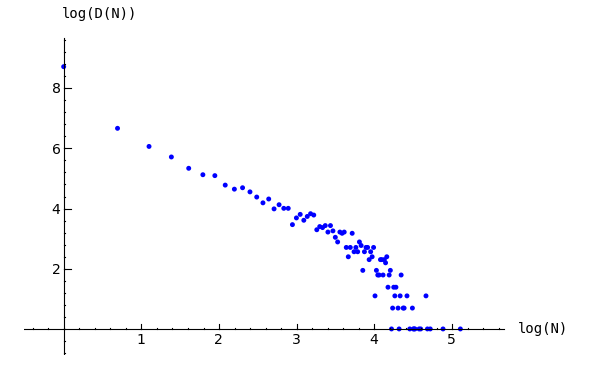
\includegraphics{btw.png}
\caption{Distribution of avalanche sizes}\end{figure}

Note: In the above code, \code{m.stabilize(true)} returns a list consisting of the
stabilized configuration and the firing vector.  (Omitting \code{true} would give
just the stabilized configuration.)
\hypertarget{discrete-riemann-surfaces}{}

\section{Divisors and Discrete Riemann surfaces}

A reference for this section is \emph{Riemann-Roch and Abel-Jacobi theory on a finite
graph} {[}BN{]}.

A \emph{divisor} on $\Gamma$ is an element of the free abelian group on its
vertices, including the sink.  Suppose, as above, that the $n+1$ vertices of
$\Gamma$ have been ordered, and that $\mathcal{L}$ is the column span of the
transpose of the Laplacian.  A divisor is then identified with an element
$D\in\mathbb{Z}^{n+1}$ and two divisors are \emph{linearly equivalent} if they
differ by an element of $\mathcal{L}$.  A divisor $E$ is \emph{effective}, written
$E\geq0$, if $E(v)\geq0$ for each $v\in V$, i.e., if $E\in\mathbb{N}^{n+1}$.
The \emph{degree} of a divisor, $D$, is $deg(D) := \sum_{v\in V}D(v)$.   The
divisors of degree zero modulo linear equivalence form the \emph{Picard group}, or
\emph{Jacobian} of the graph. For an undirected graph, the Picard group is
isomorphic to the sandpile group.

The \emph{complete linear system} for a divisor $D$, denoted $|D|$, is the
collection of effective divisors linearly equivalent to $D.$


\subsection{Riemann-Roch}

To describe the Riemann-Roch theorem in this context, suppose that $\Gamma$ is
an undirected, unweighted graph. The \emph{dimension}, $r(D)$ of the linear system
$|D|$ is $-1$ if $|D|=\emptyset$ and otherwise is the greatest integer $s$ such
that $|D-E|\neq0$ for all effective divisors $E$ of degree $s$.  Define the
\emph{canonical divisor} by $K=\sum_{v\in V}(\deg(v)-2)v$ and the \emph{genus} by $g =
|E| - |V| + 1$.  The Riemann-Roch theorem says that for any divisor $D$,
\begin{gather}
\begin{split}r(D)-r(K-D)=\deg(D)+1-g.\end{split}\notag
\end{gather}
\textbf{Example.} (Some of the following calculations require the installation of \emph{4ti2}.)

\begin{Verbatim}[commandchars=@\[\]]
The sandpile on the complete graph on 5 vertices:

    sage: G = complete@_sandpile(5)

The genus (num@_edges method counts each undirected edge twice):

    sage: g = G.num@_edges()/2 - G.num@_verts() + 1

A divisor on the graph:

    sage: D = Divisor(G, @PYGZlb[]1,2,2,0,2@PYGZrb[])

Verify the Riemann-Roch theorem:

    sage: K = G.canonical@_divisor()
    sage: D.r@_of@_D() - (K - D).r@_of@_D() == D.deg() + 1 - g
    True

The effective divisors linearly equivalent to D:

    sage: @PYGZlb[]E.values() for E in D.effective@_div()@PYGZrb[]
    @PYGZlb[]@PYGZlb[]0, 1, 1, 4, 1@PYGZrb[], @PYGZlb[]4, 0, 0, 3, 0@PYGZrb[], @PYGZlb[]1, 2, 2, 0, 2@PYGZrb[]@PYGZrb[]

The nonspecial divisors up to linear equivalence (divisors of degree
g-1 with empty linear systems)

    sage: N = G.nonspecial@_divisors()
    sage: @PYGZlb[]E.values() for E in N@PYGZlb[]:5@PYGZrb[]@PYGZrb[]   @# the first few

    @PYGZlb[]@PYGZlb[]-1, 2, 1, 3, 0@PYGZrb[],
     @PYGZlb[]-1, 0, 3, 1, 2@PYGZrb[],
     @PYGZlb[]-1, 2, 0, 3, 1@PYGZrb[],
     @PYGZlb[]-1, 3, 1, 2, 0@PYGZrb[],
     @PYGZlb[]-1, 2, 0, 1, 3@PYGZrb[]@PYGZrb[]
    sage: len(N)
    24
    sage: len(N) == G.h@_vector()@PYGZlb[]-1@PYGZrb[]
    True
\end{Verbatim}


\subsection{Picturing linear systems}

Fix a divisor $D$.  There are at least two natural graphs associated with
linear system associated with $D$.  First, consider the directed graph with
vertex set $|D|$ and with an edge from vertex $E$ to vertex $F$ if $F$ is
attained from $E$ by firing a single unstable vertex.

\begin{Verbatim}[commandchars=@\[\]]
sage: S = Sandpile(graphs.CycleGraph(6),0)
sage: D = Divisor(S, @PYGZlb[]1,1,1,1,2,0@PYGZrb[])
sage: D.is@_alive()
True
sage: eff = D.effective@_div()
sage:
firing@_graph(S,eff).show3d(edge@_size=.005,vertex@_size=0.01,iterations=500)
\end{Verbatim}
\begin{figure}[htbp]
\centering

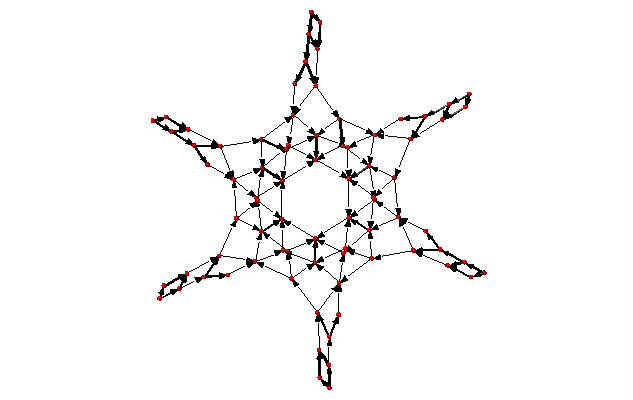
\includegraphics{C_6.png}
\caption{Complete linear system for (1,1,1,1,2,0) on $C_6$: single firings}\end{figure}

The second graph has the same set of vertices but with an edge from $E$ to $F$
if $F$ is obtained from $E$ by firing all unstable vertices of $E$.

\begin{Verbatim}[commandchars=@\[\]]
sage: S = Sandpile(graphs.CycleGraph(6),0)
sage: D = Divisor(S, @PYGZlb[]1,1,1,1,2,0@PYGZrb[])
sage: eff = D.effective@_div()
sage: parallel@_firing@_graph(S,eff).show3d(edge@_size=.005,vertex@_size=0.01,iterations=500)
\end{Verbatim}
\begin{figure}[htbp]
\centering

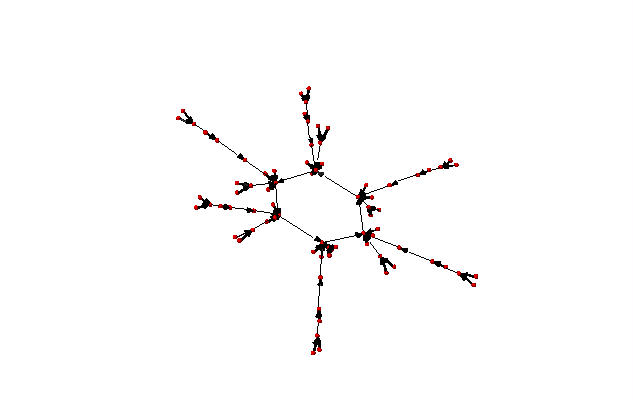
\includegraphics{C_6-parallel.png}
\caption{Complete linear system for (1,1,1,1,2,0) on $C_6$: parallel firings}\end{figure}

Note that in each of the examples, above, starting at any divisor in the linear
system and following edges, one is eventually led into a cycle of length 6
(cycling the divisor (1,1,1,1,2,0)).  Thus, \code{D.alive()} returns \code{True}.  In
Sage, one would be able to rotate the above figures to get a better idea of the
structure.


\section{Algebraic geometry of sandpiles}

A reference for the following material is in the works {[}PPW{]}.


\subsection{Affine}

Let $n=|V|-1$, and fix an ordering on the nonsink vertices of $\Gamma$.  let
$\tilde{\mathcal{L}}\subset\mathbb{Z}^n$ denote the column-span of
$\tilde{L}^t$, the transpose of the reduced Laplacian.  Label vertex $i$ with the
indeterminate $x_i$, and let $\mathbb{C}[\Gamma_s] = \mathbb{C}[x_1,\dots,x_n]$.
(Here, $s$ denotes the sink vertex of $\Gamma$.) The \emph{sandpile ideal} or
\emph{toppling ideal} is the lattice ideal for $\tilde{\mathcal{L}}$:
\begin{gather}
\begin{split}I = I(\Gamma_s) := \{x^u-x^v: u-v
\tilde{\mathcal{L}}\}\subset\mathbb{C}[\Gamma_s],\end{split}\notag
\end{gather}
where $x^u := \prod_{i=1}^nx^{u_i}$ for $u\in\mathbb{Z}^n$.

For each $c\in\mathbb{Z}^n$ define $t(c) = x^{c^+} - x^{c^-}$ where
$c^+_i=\max\{c_i,0\}$ and $c^-=\max\{-c_i,0\}$ so that $c=c^+-c^-$.
Then, for each $\sigma\in\mathbb{Z}^n$, define $T(\sigma) =
t(\tilde{L}^t\sigma)$.  It then turns out that
\begin{gather}
\begin{split}I = (T(e_1),\dots,T(e_n),x^b-1)\end{split}\notag
\end{gather}
where $e_i$ is the $i$-th standard basis vector and $b$ is any burning
configuration.

The affine coordinate ring, $\mathbb{C}[\Gamma_s]/I,$ is isomorphic to the group
algebra of the sandpile group, $\mathbb{C}[\mathcal{S}(\Gamma)].$

The standard term-ordering on $\mathbb{C}[\Gamma_s]$ is graded reverse
lexigraphical order with $x_i>x_j$ if vertex $v_i$ is further from the sink than
vertex $v_j$.  If $\sigma_b$ is the script for a burning configuration (not
necessarily minimal), then
\begin{gather}
\begin{split}\{T(\sigma): \sigma\leq\sigma_b\}\end{split}\notag
\end{gather}
is a Groebner basis for $I$.


\subsection{Projective}

Now let $\mathbb{C}[\Gamma]=\mathbb{C}[x_0,x_1,\dots,x_n]$, where $x_0$
corresponds to the sink vertex.  The \emph{homogeneous sandpile ideal}, denoted
$I^h$, is obtaining by homogenizing $I$ with respect to $x_0$.  Let $L$ be the
(full) Laplacian, and $\mathcal{L}\subset\mathbb{Z}^{n+1}$ be the column span of
its transpose, $L^t.$  Then $I^h$ is the lattice ideal for $\mathcal{L}$:
\begin{gather}
\begin{split}I^h = I^h(\Gamma) := \{x^u-x^v: u-v \in\mathcal{L}\}\subset\mathbb{C}[\Gamma].\end{split}\notag
\end{gather}
This ideal can be calculated by saturating the ideal
\begin{gather}
\begin{split}(T(e_i): i=0,\dots n)\end{split}\notag
\end{gather}
with respect to the product of the indeterminates: $\prod_{i=0}^nx_i$ (extending
the $T$ operator in the obvious way).  A Groebner basis with respect to the
degree lexicographic order describe above (with $x_0$ the smallest vertex), is
obtained by homogenizing each element of the Groebner basis for the
non-homogeneous sandpile ideal with respect to $x_0.$

\textbf{Example.}

\begin{Verbatim}[commandchars=@\[\]]
    sage: g = {0:{},1:{0:1,3:1,4:1},2:{0:1,3:1,5:1},
               3:{2:1,5:1},4:{1:1,3:1},5:{2:1,3:1}}
    sage: S = Sandpile(g, 0)
    sage: S.ring()

    //   characteristic : 0
    //   number of vars : 6
    //        block   1 : ordering dp
    //                  : names    x@_5 x@_4 x@_3 x@_2 x@_1 x@_0
    //        block   2 : ordering C

The homogeneous sandpile ideal:

    sage: S.ideal()
    x@_2-x@_0,
    x@_3@textasciicircum[]2-x@_5*x@_0,
    x@_5*x@_3-x@_0@textasciicircum[]2,
    x@_4@textasciicircum[]2-x@_3*x@_1,
    x@_5@textasciicircum[]2-x@_3*x@_0,
    x@_1@textasciicircum[]3-x@_4*x@_3*x@_0,
    x@_4*x@_1@textasciicircum[]2-x@_5*x@_0@textasciicircum[]2

its resolution:

    sage: S.resolution()
    'R @textless[]-- R@textasciicircum[]7 @textless[]-- R@textasciicircum[]19 @textless[]-- R@textasciicircum[]25 @textless[]-- R@textasciicircum[]16 @textless[]-- R@textasciicircum[]4'

and Betti table:

    sage: S.betti()
               0     1     2     3     4     5
    ------------------------------------------
        0:     1     1     -     -     -     -
        1:     -     4     6     2     -     -
        2:     -     2     7     7     2     -
        3:     -     -     6    16    14     4
    ------------------------------------------
    total:     1     7    19    25    16     4

The Hilbert function:

    sage: S.hilbert@_function()
    @PYGZlb[]1, 5, 11, 15@PYGZrb[]

and its first differences (which counts the number of superstable
configurations in each degree):

    sage: S.first@_diffs@_hilb()
    @PYGZlb[]1, 4, 6, 4@PYGZrb[]
    sage: x = @PYGZlb[]sum(i) for i in S.superstables(False)@PYGZrb[]
    sage: sorted(x)
    @PYGZlb[]0, 1, 1, 1, 1, 2, 2, 2, 2, 2, 2, 3, 3, 3, 3@PYGZrb[]

The degree in which the Hilbert function equals the Hilbert polynomial, the
latter always being a constant in the case of a sandpile ideal:

    sage: S.postulation()
    3
\end{Verbatim}


\subsection{Zeros}

The \emph{zero set} for the sandpile ideal $I$ is
\begin{gather}
\begin{split}Z(I) = \{p\in\mathbb{C}^n: f(p)=0\mbox{ for all $f\in I$}\},\end{split}\notag
\end{gather}
the set of simultaneous zeros of the polynomials in $I.$  Letting $S^1$ denote
the unit circle in the complex plane, $Z(I)$ is a finite
subgroup of $S^1\times\dots\times S^1\subset\mathbb{C}^n$, isomorphic to the
sandpile group.  The zero set is actually linearly isomorphic to a faithful representation of the sandpile group on $\mathbb{C}^n.$

\textbf{Example.} (Continued.)

\begin{Verbatim}[commandchars=@\[\]]
     sage: S = Sandpile({0: {}, 1: {2: 2}, 2: {0: 4, 1: 1}}, 0)
     sage: S.ideal()
     x@_1@textasciicircum[]2-x@_2@textasciicircum[]2,
     x@_1*x@_2@textasciicircum[]3-x@_0@textasciicircum[]4,
     x@_2@textasciicircum[]5-x@_1*x@_0@textasciicircum[]4

Approximation to the zero set (setting []`[]`x@_0 = 1[]`[]`):

     sage: S.solve()

     @PYGZlb[]@PYGZlb[]0.707107*I - 0.707107, 0.707107 - 0.707107*I@PYGZrb[],
      @PYGZlb[]-0.707107*I - 0.707107, 0.707107*I + 0.707107@PYGZrb[],
      @PYGZlb[]-1*I, -1*I@PYGZrb[],
      @PYGZlb[]I, I@PYGZrb[],
      @PYGZlb[]0.707107*I + 0.707107, -0.707107*I - 0.707107@PYGZrb[],
      @PYGZlb[]0.707107 - 0.707107*I, 0.707107*I - 0.707107@PYGZrb[],
      @PYGZlb[]1, 1@PYGZrb[],
      @PYGZlb[]-1, -1@PYGZrb[]@PYGZrb[]
     sage: len(@_) == S.group@_order()
     True

 The zeros are generated as a group by a single vector:

     sage: S.points()
     @PYGZlb[]@PYGZlb[]e@textasciicircum[](1/4*I*pi), e@textasciicircum[](-3/4*I*pi)@PYGZrb[]@PYGZrb[]
\end{Verbatim}
\hypertarget{installation}{}

\subsection{Complete Intersections and Arithmetically Gorenstein toppling ideals}

To do.


\subsection{Resolutions}

The homogeneous sandpile ideal, $I^h$, has a free resolution graded by the
divisors on $\Gamma$ modulo linear equivalence.  (See the section on
\emph{Discrete Riemann Surfaces} for the language of
divisors and linear equivalence.)  Let
$S=\mathbb{C}[\Gamma]=\mathbb{C}[x_0,\dots,x_n]$, as above, and let
$\mathfrak{S}$ denote the group of divisors modulo rational equivalence.  Then
$S$ is graded by $\mathfrak{S}$ by letting $\deg(x^c)= c\in\mathfrak{S}$ for
each monomial $x^c$.  The minimal free resolution of $I^h$ has the form
\begin{gather}
\begin{split} 0\leftarrow I^h
\leftarrow\oplus_{D\in\mathfrak{S}}S(-D)^{\beta_{0,D}}\leftarrow\oplus_{D\in\mathfrak{S}}S(-D)^{\beta_{1,D}}
\leftarrow\dots\leftarrow\oplus_{D\in\mathfrak{S}}S(-D)^{\beta_{r,D}}\leftarrow0.\end{split}\notag
\end{gather}
where the $\beta_{i,D}$ are the \emph{Betti numbers} for $I^h$.

For each divisor class $D\in\mathfrak{S}$, define a simplicial complex,
\begin{gather}
\begin{split}\Delta_D := \{I\subseteq\{0,\dots,n\}: I\subseteq\mbox{supp}(E)\mbox{ for some}\
E\in |D|\}.\end{split}\notag
\end{gather}
The Betti number $\beta_{i,D}$ equals the dimension over $\mathbb{C}$ of the
$i$-th reduced homology group of $\Delta_D$:
\begin{gather}
\begin{split}\beta_{i,D} = \dim_{\mathbb{C}}\tilde{H}_i(\Delta_D;\mathbb{C}).\end{split}\notag
\end{gather}
\begin{Verbatim}[commandchars=@\[\]]
        sage: S = Sandpile({0:{},1:{0: 1, 2: 1, 3: 4},2:{3: 5},3:{1: 1, 2: 1}},0)

Representatives of all divisor classes with nontrivial homology:

    sage: p = S.betti@_complexes()
    sage: p@PYGZlb[]0@PYGZrb[]
    @PYGZlb[]{0: -8, 1: 5, 2: 4, 3: 1},
     Simplicial complex with vertex set (0, 1, 2, 3) and facets {(1, 2), (3,)}@PYGZrb[]

The homology associated with the first divisor in the list:

    sage: D = p@PYGZlb[]0@PYGZrb[]@PYGZlb[]0@PYGZrb[]
    sage: S.effective@_div(D)
    @PYGZlb[]{0: 0, 1: 1, 2: 1, 3: 0}, {0: 0, 1: 0, 2: 0, 3: 2}@PYGZrb[]
    sage: @PYGZlb[]S.support(E) for E in S.effective@_div(D)@PYGZrb[]
    @PYGZlb[]@PYGZlb[]1, 2@PYGZrb[], @PYGZlb[]3@PYGZrb[]@PYGZrb[]
    sage: S.Dcomplex(D)
    Simplicial complex with vertex set (0, 1, 2, 3) and facets {(1, 2), (3,)}
    sage: S.Dcomplex(D).homology()
    {0: Z, 1: 0}


The minimal free resolution:

    sage: S.resolution()
    'R @textless[]-- R@textasciicircum[]5 @textless[]-- R@textasciicircum[]5 @textless[]-- R@textasciicircum[]1'
    sage: S.betti()
               0     1     2     3
    ------------------------------
        0:     1     -     -     -
        1:     -     5     5     -
        2:     -     -     -     1
    ------------------------------
    total:     1     5     5     1
    sage: len(p)
    11

The degrees and ranks of the homology groups foreach element of the list p (compare with the
Betti table, above):

    sage: @PYGZlb[]@PYGZlb[]sum(d@PYGZlb[]0@PYGZrb[].values()),d@PYGZlb[]1@PYGZrb[].betti()@PYGZrb[] for d in p@PYGZrb[]

    @PYGZlb[]@PYGZlb[]2, {0: 1, 1: 0}@PYGZrb[],
     @PYGZlb[]3, {0: 0, 1: 1, 2: 0}@PYGZrb[],
     @PYGZlb[]2, {0: 1, 1: 0}@PYGZrb[],
     @PYGZlb[]3, {0: 0, 1: 1, 2: 0}@PYGZrb[],
     @PYGZlb[]2, {0: 1, 1: 0}@PYGZrb[],
     @PYGZlb[]3, {0: 0, 1: 1, 2: 0}@PYGZrb[],
     @PYGZlb[]2, {0: 1, 1: 0}@PYGZrb[],
     @PYGZlb[]3, {0: 0, 1: 1}@PYGZrb[],
     @PYGZlb[]2, {0: 1, 1: 0}@PYGZrb[],
     @PYGZlb[]3, {0: 0, 1: 1, 2: 0}@PYGZrb[],
     @PYGZlb[]5, {0: 0, 1: 0, 2: 1}@PYGZrb[]@PYGZrb[]
\end{Verbatim}

TODO: Add section on the Betti numbers of undirected graphs.


\chapter{Installation}

It is assumed that Sage is already installed.  If not, please see
the main \href{http://www.sagemath.org}{Sage homepage} for installation instructions.
To use \code{sandpile.sage}:
\begin{itemize}
\item {} 
download \href{http://www.reed.edu/\textasciitilde{}davidp/sand}{sandpile.sage}

\item {} 
start Sage, and issue the command

\end{itemize}

\begin{Verbatim}[commandchars=@\[\]]
sage: load sandpile.sage
\end{Verbatim}

You may need to give the full path name to \code{sandpile.sage}.

\begin{notice}{warning}{Warning:}
The methods for computing linear systems of divisors and their corresponding
simplicial complexes require the installation of 4ti2.
\end{notice}

To make 4ti2 usable from Sage Sandpiles there are two options:
\begin{enumerate}
\item {} 
Go to the \href{http://sagemath.org/download-packages.html}{Sage website} and
look for the precise names of the glpk and 4ti2 packages and install them
according to the instructions given there.  For instance, suppose the glpk
package is named glpk-4.9.spkg.  Install the package with the following
command from a UNIX shell prompt:

\end{enumerate}

\begin{Verbatim}[commandchars=@\[\]]
sage -i glpk-4.9
\end{Verbatim}
\begin{enumerate}
\item {} 
Download the program from the \href{http://www.4ti2.de/}{4ti2 homepage}, and

\end{enumerate}
\begin{quote}

follow the installation instructions given there.
\end{quote}
\begin{itemize}
\item {} 
open \code{sandpiles.sage} in your favorite text editor and edit the following
line (near the beginning of the file, near the copyright statement and the
start of the definition of the Sandpile class), replacing the
\code{path\_to\_zsolve} string with the path to the executables in \emph{your} 4ti2
directory:

\end{itemize}

\begin{Verbatim}[commandchars=@\[\]]
@PYG[n][path@_to@_zsolve] @PYG[o][=] @PYG[l+s][']@PYG[l+s][/home/davidp/math/sandpile/4ti2/linux@_x86/]@PYG[l+s][']
\end{Verbatim}
\begin{itemize}
\item {} 
start Sage and load \code{sandpiles.sage} as described above.

\end{itemize}


\chapter{Usage}


\section{Initialization}

Most of \code{sandpile.sage} consists of the definition of the classes
\code{Sandpile}, \code{Config}, and \code{Divisor}.
Initialization for \code{Sandpile} has the form

\begin{Verbatim}[commandchars=@\[\]]
sage: S = Sandpile(graph, sink)
\end{Verbatim}

where \code{graph} represents a graph and \code{sink} is the key for the sink
vertex.  There are four possible forms for \code{graph}:
\begin{enumerate}
\item {} 
a Python dictionary of dictionaries:

\end{enumerate}

\begin{Verbatim}[commandchars=@\[\]]
sage: g = {0: {}, 1: {0: 1, 3: 1, 4: 1}, 2: {0: 1, 3: 1, 5: 1},
           3: {2: 1, 5: 1}, 4: {1: 1, 3: 1}, 5: {2: 1, 3: 1}}
\end{Verbatim}
\begin{figure}[htbp]
\centering

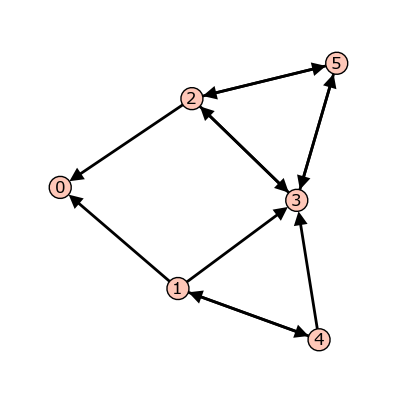
\includegraphics{initial.png}
\caption{Graph from dictionary of dictionaries.}\end{figure}

Each key is the name of a vertex.  Next to each vertex name $v$ is a dictionary
consisting of pairs: \code{vertex: weight}.  Each pair represents a directed edge
emanating from $v$ and ending at \code{vertex} having (non-negative integer) weight
equal to \code{weight}.  Loops are allowed. In the example above, all of the weights are 1.
\begin{enumerate}
\item {} 
a Python dictionary of lists:

\end{enumerate}

\begin{Verbatim}[commandchars=@\[\]]
sage: g = {0: @PYGZlb[]@PYGZrb[], 1: @PYGZlb[]0, 3, 4@PYGZrb[], 2: @PYGZlb[]0, 3, 5@PYGZrb[],
           3: @PYGZlb[]2, 5@PYGZrb[], 4: @PYGZlb[]1, 3@PYGZrb[], 5: @PYGZlb[]2, 3@PYGZrb[]}
\end{Verbatim}

This is a short-hand when all of the edge-weights are equal to 1.  The above
example is for the same displayed graph.
\begin{enumerate}
\item {} 
a Sage graph (of type \code{sage.graphs.graph.Graph}):

\end{enumerate}

\begin{Verbatim}[commandchars=@\[\]]
sage: g = graphs.CycleGraph(5)
sage: S = Sandpile(g, 0)
sage: type(g)
@textless[]class 'sage.graphs.graph.Graph'@textgreater[]
\end{Verbatim}

To see the types of built-in graphs, type \code{graphs.}, including the period,
and hit TAB.
\begin{enumerate}
\item {} 
a Sage digraph:

\end{enumerate}

\begin{Verbatim}[commandchars=@\[\]]
sage: S = Sandpile(digraphs.RandomDirectedGNC(6), 0)
sage: S.show()
\end{Verbatim}
\begin{figure}[htbp]
\centering

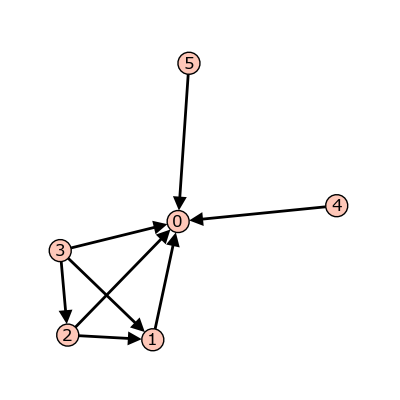
\includegraphics{random.png}
\caption{A random graph.}\end{figure}

See \href{http://sagemath.org/doc/reference/sage/graphs/graph\_generators.html}{http://sagemath.org/doc/reference/sage/graphs/graph\_generators.html} for
more information on the Sage graph library and graph constructors.

Each of these four formats is preprocessed by the Sandpile class so that,
internally, the graph is represented by the dictionary of dictionaries format
first presented.  This internal format is returned by  \code{dict()}:

\begin{Verbatim}[commandchars=@\[\]]
sage: S  = Sandpile({0:@PYGZlb[]@PYGZrb[], 1:@PYGZlb[]0, 3, 4@PYGZrb[], 2:@PYGZlb[]0, 3, 5@PYGZrb[],
                     3: @PYGZlb[]2, 5@PYGZrb[], 4: @PYGZlb[]1, 3@PYGZrb[], 5: @PYGZlb[]2, 3@PYGZrb[]},0)
sage: S.dict()

{0: {},
 1: {0: 1, 3: 1, 4: 1},
 2: {0: 1, 3: 1, 5: 1},
 3: {2: 1, 5: 1},
 4: {1: 1, 3: 1},
 5: {2: 1, 3: 1}}
\end{Verbatim}

\begin{notice}{note}{Note:}
The user is responsible for assuring that each vertex has a directed path
into the designated sink.  If the sink has out-edges, these will be ignored
for the purposes of sandpile calculations (but not calculations on divisors).
\end{notice}

\textbf{Code for checking whether a given vertex is a sink:}

\begin{Verbatim}[commandchars=@\[\]]
sage:  S  = Sandpile({0:@PYGZlb[]@PYGZrb[], 1:@PYGZlb[]0, 3, 4@PYGZrb[], 2:@PYGZlb[]0, 3, 5@PYGZrb[],
                         3: @PYGZlb[]2, 5@PYGZrb[], 4: @PYGZlb[]1, 3@PYGZrb[], 5: @PYGZlb[]2, 3@PYGZrb[]},0)
sage: @PYGZlb[]S.distance(v,0) for v in S.vertices()@PYGZrb[] @# 0 is a sink
@PYGZlb[]0, 1, 1, 2, 2, 2@PYGZrb[]
sage: @PYGZlb[]S.distance(v,1) for v in S.vertices()@PYGZrb[] @# 1 is not a sink
@PYGZlb[]+Infinity, 0, +Infinity, +Infinity, 1, +Infinity@PYGZrb[]
\end{Verbatim}


\section{Methods}

Here are summaries of \code{Sandpile}, \code{Config}, and \code{Divisor} methods
(functions).  Each summary is followed by a list of complete descriptions of
the methods.  There are many more methods available for a Sandpile, e.g.,
those inherited from the class DiGraph.  To see them all, enter

\begin{Verbatim}[commandchars=@\[\]]
sage: dir(Sandpile)
\end{Verbatim}

or type \code{Sandpile.}, including the period, and hit TAB.


\subsection{Sandpile}

\textbf{Summary of methods.}
\begin{itemize}
\item {} 
\emph{all\_k\_config(k)} --- The configuration with all values set to k.

\item {} 
\emph{all\_k\_div(k)} --- The divisor with all values set to k.

\item {} 
\emph{betti(verbose)} --- The Betti table for the
homogeneous sandpile ideal.

\item {} 
\emph{betti\_complexes()} --- The divisors with
nonempty linear systems along with their with their simplicial complexes.

\item {} 
\emph{burning\_config()} --- A minimal burning configuration.

\item {} 
\emph{burning\_script()} --- A script for the minimal burning configuration.

\item {} 
\emph{canonical\_divisor()} --- The canonical divisor (for undirected graphs).

\item {} 
\emph{dict()} --- A dictionary of dictionaries representing a directed graph.

\item {} 
\emph{elementary\_divisors()} --- The elementary
divisors of the sandpile group (a finite abelian group).

\item {} 
\emph{groebner()} --- Groebner basis for the homogeneous
sandpile ideal with respect to the standard sandpile ordering.

\item {} 
\emph{group\_order()} --- The size of the sandpile group.

\item {} 
\emph{h\_vector()} --- The first differences of the
Hilbert function of the homogeneous sandpile ideal.

\item {} 
\emph{hilbert\_function()} --- The Hilbert function of the homogeneous sandpile ideal.

\item {} 
\emph{ideal()} --- The saturated, homogeneous sandpile ideal.

\item {} 
\emph{identity()} --- The identity configuration.

\item {} 
\emph{in\_degree(v)} --- The in-degree of a vertex or a list of all in-degrees.

\item {} 
\emph{is\_undirected()} --- \code{True} if \code{(u,v)} is and edge if and only if \code{(v,u)} is an edges, each edge with the same weight.

\item {} 
\emph{laplacian()} --- The Laplacian matrix of the graph.

\item {} 
\emph{max\_stable()} --- The maximal stable configuration.

\item {} 
\emph{max\_stable\_div()} --- The maximal stable divisor.

\item {} 
\emph{max\_superstables()} --- The maximal superstable
configurations.

\item {} 
\emph{min\_recurrents()} --- The minimal recurrent
elements.

\item {} 
\emph{nonsink\_vertices()} --- The names of the nonsink vertices.

\item {} 
\emph{nonspecial\_divisors()} --- The nonspecial
divisors (only for undirected graphs).

\item {} 
\emph{num\_edges()} --- The number of edges.

\item {} 
\emph{out\_degree(v)} --- The out-degree of a vertex or a list of all out-degrees.

\item {} 
\emph{points()} --- Generators for the multiplicative group of
zeros of the sandpile ideal.

\item {} 
\emph{postulation()} --- The postulation number of the sandpile ideal.

\item {} 
\emph{recurrents(verbose)} --- The list of recurrent
configurations.

\item {} 
\emph{reduced\_laplacian()} --- The reduced Laplacian matrix of the graph.

\item {} 
\emph{reorder\_vertices()} --- Create a copy of the
sandpile but with the vertices reordered

\item {} 
\emph{resolution(verbose)} --- The
minimal free resolution of the homogeneous sandpile ideal.

\item {} 
\emph{ring()} --- The ring containing the homogeneous sandpile ideal.

\item {} 
\emph{sink()} --- The identifier for the sink vertex.

\item {} 
\emph{solve()} --- Approximations of the complex affine zeros of the sandpile ideal.

\item {} 
\emph{superstables(verbose)} --- The list of
superstable configurations.

\item {} 
\emph{symmetric\_recurrents(orbits)} --- The list of symmetric recurrent configurations.

\item {} 
\emph{unsaturated\_ideal()} --- The unsaturated, homogeneous sandpile ideal.

\item {} 
\emph{version()} --- The version number of Sage Sandpiles.

\item {} 
\emph{vertices(boundary\_first)} --- The list

\item {} 
\emph{zero\_config()} --- The all-zero configuration.

\item {} 
\emph{zero\_div()} --- The all-zero divisor.

\end{itemize}


\bigskip\hrule{}\bigskip


\textbf{Complete descriptions of Sandpile methods.}

---
\hypertarget{all-k-config-k}{}
\textbf{all\_k\_config(k)}
\begin{quote}

The configuration with all values set to k.

INPUT:

\code{k} - integer

OUTPUT:

Config

EXAMPLES:

\begin{Verbatim}[commandchars=@\[\]]
sage: S = sandlib('generic')
sage: S.all@_k@_config(7)
{1: 7, 2: 7, 3: 7, 4: 7, 5: 7}
\end{Verbatim}
\end{quote}

---
\hypertarget{all-k-div-k}{}
\textbf{all\_k\_div(k)}
\begin{quote}

The divisor with all values set to k.

INPUT:

\code{k} - integer

OUTPUT:

Divisor

EXAMPLES:

\begin{Verbatim}[commandchars=@\[\]]
sage: S = sandlib('generic')
sage: S.all@_k@_div(7)
{0: 7, 1: 7, 2: 7, 3: 7, 4: 7, 5: 7}
\end{Verbatim}
\end{quote}

---
\hypertarget{betti-verbose}{}
\textbf{betti(verbose)}
\begin{quote}

Computes the Betti table for the homogeneous sandpile ideal.  If
\code{verbose} is \code{True}, it prints the standard Betti table, otherwise,
it returns a less formated table.

INPUT:

\code{verbose} (optional) - boolean

OUTPUT:

Betti numbers for the sandpile

EXAMPLES:

\begin{Verbatim}[commandchars=@\[\]]
sage: S = sandlib('generic')
sage: S.betti()
           0     1     2     3     4     5
------------------------------------------
    0:     1     1     -     -     -     -
    1:     -     4     6     2     -     -
    2:     -     2     7     7     2     -
    3:     -     -     6    16    14     4
------------------------------------------
total:     1     7    19    25    16     4
\end{Verbatim}
\end{quote}

---
\hypertarget{betti-complexes}{}
\textbf{betti\_complexes()}
\begin{quote}

Returns a list of all the divisors with nonempty linear systems whose
corresponding simplicial complexes have nonzero homology in some
dimension. Each such divisors is returned with its corresponding
simplicial complex.

INPUT:

None

OUTPUT:

list (of pairs {[}divisors, corresponding simplicial complex{]})

EXAMPLES:

\begin{Verbatim}[commandchars=@\[\]]
sage: S = Sandpile({0:{},1:{0: 1, 2: 1, 3: 4},2:{3: 5},3:{1: 1, 2: 1}},0)
sage: p = S.betti@_complexes()
sage: p@PYGZlb[]0@PYGZrb[]
@PYGZlb[]{0: -8, 1: 5, 2: 4, 3: 1},
 Simplicial complex with vertex set (0, 1, 2, 3) and facets {(1, 2), (3,)}@PYGZrb[]
sage: S.resolution()
'R @textless[]-- R@textasciicircum[]5 @textless[]-- R@textasciicircum[]5 @textless[]-- R@textasciicircum[]1'
sage: S.betti()
           0     1     2     3
------------------------------
    0:     1     -     -     -
    1:     -     5     5     -
    2:     -     -     -     1
------------------------------
total:     1     5     5     1
sage: len(p)
11
sage: p@PYGZlb[]0@PYGZrb[]@PYGZlb[]1@PYGZrb[].homology()
{0: Z, 1: 0}
sage: p@PYGZlb[]-1@PYGZrb[]@PYGZlb[]1@PYGZrb[].homology()
{0: 0, 1: 0, 2: Z}
\end{Verbatim}
\end{quote}

---
\hypertarget{burning-config}{}
\textbf{burning\_config()}
\begin{quote}

A minimal burning configuration.

INPUT:

None

OUTPUT:

dict (configuration)

EXAMPLES:

\begin{Verbatim}[commandchars=@\[\]]
sage: g = {0:{},1:{0:1,3:1,4:1},2:{0:1,3:1,5:1},
           3:{2:1,5:1},4:{1:1,3:1},5:{2:1,3:1}}
sage: S = Sandpile(g,0)
sage: S.burning@_config()
{1: 2, 2: 0, 3: 1, 4: 1, 5: 0}
sage: S.burning@_config().values()
@PYGZlb[]2, 0, 1, 1, 0@PYGZrb[]
sage: S.burning@_script()
{1: 1, 2: 3, 3: 5, 4: 1, 5: 4}
sage: script = S.burning@_script().values()
sage: script
@PYGZlb[]1, 3, 5, 1, 4@PYGZrb[]
sage: matrix(script)*S.reduced@_laplacian()
@PYGZlb[]2 0 1 1 0@PYGZrb[]
\end{Verbatim}

NOTES:

The burning configuration and script are computed using a modified
version of Speer's script algorithm.  This is a generalization to
directed multigraphs of Dhar's burning algorithm.

A \emph{burning configuration} is a nonnegative integer-linear
combination of the rows of the reduced Laplacian matrix having
nonnegative entries and such that every vertex has a path from some
vertex in its support.  The corresponding \emph{burning script} gives
the integer-linear combination needed to obtain the burning
configuration.  So if $b$ is the burning configuration, $sigma$ is its
script, and $tilde{L}$ is the reduced Laplacian, then $sigma *
tilde{L} = b$.  The \emph{minimal burning configuration} is the one
with the minimal script (its components are no larger than the
components of any other script
for a burning configuration).

The following are equivalent for a configuration $c$ with burning
configuration $b$ having script $sigma$:
\begin{itemize}
\item {} 
$c$ is recurrent;

\item {} 
$c+b$ stabilizes to $c$;

\item {} 
the firing vector for the stabilization of $c+b$ is $sigma$.

\end{itemize}
\end{quote}

---
\hypertarget{burning-script}{}
\textbf{burning\_script()}
\begin{quote}

A script for the minimal burning configuration.

INPUT:

None

OUTPUT:

dict

EXAMPLES:

\begin{Verbatim}[commandchars=@\[\]]
sage: g = {0:{},1:{0:1,3:1,4:1},2:{0:1,3:1,5:1},
           3:{2:1,5:1},4:{1:1,3:1},5:{2:1,3:1}}
sage: S = Sandpile(g,0)
sage: S.burning@_config()
{1: 2, 2: 0, 3: 1, 4: 1, 5: 0}
sage: S.burning@_config().values()
@PYGZlb[]2, 0, 1, 1, 0@PYGZrb[]
sage: S.burning@_script()
{1: 1, 2: 3, 3: 5, 4: 1, 5: 4}
sage: script = S.burning@_script().values()
sage: script
@PYGZlb[]1, 3, 5, 1, 4@PYGZrb[]
sage: matrix(script)*S.reduced@_laplacian()
@PYGZlb[]2 0 1 1 0@PYGZrb[]
\end{Verbatim}

NOTES:

The burning configuration and script are computed using a modified
version of Speer's script algorithm.  This is a generalization to
directed multigraphs of Dhar's burning algorithm.

A \emph{burning configuration} is a nonnegative integer-linear
combination of the rows of the reduced Laplacian matrix having
nonnegative entries and such that every vertex has a path from some
vertex in its support.  The corresponding \emph{burning script} gives the
integer-linear combination needed to obtain the burning configuration.
So if $b$ is the burning configuration, $s$ is its script, and
$L_{mathrm{red}}$ is the reduced Laplacian, then $s *
L_{mathrm{red}}= b$.  The \emph{minimal burning configuration} is the one
with the minimal script (its components are no larger than the
components of any other script
for a burning configuration).

The following are equivalent for a configuration $c$ with burning
configuration $b$ having script $s$:
\begin{itemize}
\item {} 
$c$ is recurrent;

\item {} 
$c+b$ stabilizes to $c$;

\item {} 
the firing vector for the stabilization of $c+b$ is $s$.

\end{itemize}
\end{quote}

---
\hypertarget{canonical-divisor}{}
\textbf{canonical\_divisor()}
\begin{quote}

Returns the canonical divisor: the divisor \code{deg(v)-2} grains of sand
on each vertex.  Only for undirected graphs.

INPUT:

None

OUTPUT:

Divisor

EXAMPLES:

\begin{Verbatim}[commandchars=@\[\]]
sage: S = complete@_sandpile(4)
sage: S.canonical@_divisor()
{0: 1, 1: 1, 2: 1, 3: 1}
\end{Verbatim}
\end{quote}

---
\hypertarget{dict}{}
\textbf{dict()}
\begin{quote}

Returns a dictionary of dictionaries representing a directed graph.

INPUT:

None

OUTPUT:

dict

EXAMPLES:

\begin{Verbatim}[commandchars=@\[\]]
sage: G = sandlib('generic')
sage: G.dict()
{0: {},
 1: {0: 1, 3: 1, 4: 1},
 2: {0: 1, 3: 1, 5: 1},
 3: {2: 1, 5: 1},
 4: {1: 1, 3: 1},
 5: {2: 1, 3: 1}}
sage: G.sink()
0
\end{Verbatim}
\end{quote}

---
\hypertarget{elementary-divisors}{}
\textbf{elementary\_divisors()}
\begin{quote}

The elementary divisors of the sandpile group (a finite
abelian group).

INPUT:

None

OUTPUT:

list of integers

EXAMPLES:

\begin{Verbatim}[commandchars=@\[\]]
sage: S = sandlib('generic')
sage: S.elementary@_divisors()
@PYGZlb[]1, 1, 1, 1, 15@PYGZrb[]
\end{Verbatim}
\end{quote}

---
\hypertarget{groebner}{}
\textbf{groebner()}
\begin{quote}

Returns a Groebner basis for the homogeneous sandpile ideal with
respect to the standard sandpile ordering (see \code{ring}).

INPUT:

None

OUTPUT:

Groebner basis

EXAMPLES:

\begin{Verbatim}[commandchars=@\[\]]
sage: S = sandlib('generic')
sage: S.groebner()
x@_2-x@_0,
x@_3@textasciicircum[]2-x@_5*x@_0,
x@_5*x@_3-x@_0@textasciicircum[]2,
x@_4@textasciicircum[]2-x@_3*x@_1,
x@_5@textasciicircum[]2-x@_3*x@_0,
x@_1@textasciicircum[]3-x@_4*x@_3*x@_0,
x@_4*x@_1@textasciicircum[]2-x@_5*x@_0@textasciicircum[]2
\end{Verbatim}
\end{quote}

---
\hypertarget{group-order}{}
\textbf{group\_order()}
\begin{quote}

Returns the size of the sandpile group.

INPUT:

None

OUTPUT:

int

EXAMPLES:

\begin{Verbatim}[commandchars=@\[\]]
sage: S = sandlib('generic')
sage: S.group@_order()
15
\end{Verbatim}
\end{quote}

---
\hypertarget{h-vector}{}
\textbf{h\_vector()}
\begin{quote}

Returns the first differences of the Hilbert function of the homogeneous
sandpile ideal.  It lists the number of superstable configurations in
each degree.

INPUT:

None

OUTPUT:

list of nonnegative integers

EXAMPLES:

\begin{Verbatim}[commandchars=@\[\]]
sage: S = sandlib('generic')
sage: S.hilbert@_function()
@PYGZlb[]1, 5, 11, 15@PYGZrb[]
sage: S.h@_vector()
@PYGZlb[]1, 4, 6, 4@PYGZrb[]
\end{Verbatim}
\end{quote}

---
\hypertarget{hilbert-function}{}
\textbf{hilbert\_function()}
\begin{quote}

Returns the Hilbert function of the homogeneous sandpile ideal.

INPUT:

None

OUTPUT:

list of nonnegative integers

EXAMPLES:

\begin{Verbatim}[commandchars=@\[\]]
sage: S = sandlib('generic')
sage: S.hilbert@_function()
@PYGZlb[]1, 5, 11, 15@PYGZrb[]
\end{Verbatim}
\end{quote}

---
\hypertarget{ideal}{}
\textbf{ideal()}
\begin{quote}

The saturated, homogeneous sandpile ideal.

INPUT:

None

OUTPUT:

ideal

EXAMPLES:

\begin{Verbatim}[commandchars=@\[\]]
sage: S = sandlib('generic')
sage: S.ideal()
x@_2-x@_0,
x@_3@textasciicircum[]2-x@_5*x@_0,
x@_5*x@_3-x@_0@textasciicircum[]2,
x@_4@textasciicircum[]2-x@_3*x@_1,
x@_5@textasciicircum[]2-x@_3*x@_0,
x@_1@textasciicircum[]3-x@_4*x@_3*x@_0,
x@_4*x@_1@textasciicircum[]2-x@_5*x@_0@textasciicircum[]2
\end{Verbatim}
\end{quote}

---
\hypertarget{identity}{}
\textbf{identity()}
\begin{quote}

Returns the identity configuration.

INPUT:

None

OUTPUT:

dict (the identity configuration)

EXAMPLES:

\begin{Verbatim}[commandchars=@\[\]]
sage: S = sandlib('generic')
sage: e = S.identity()
sage: x = e @& S.max@_stable()  @# stable addition
sage: x
{1: 2, 2: 2, 3: 1, 4: 1, 5: 1}
sage: x == S.max@_stable()
True
\end{Verbatim}
\end{quote}

---
\hypertarget{in-degree-v}{}
\textbf{in\_degree(v)}
\begin{quote}

Return the in-degree of a vertex or a list of all in-degrees.

INPUT:

\code{v} - vertex name or None

OUTPUT:

integer or dict

EXAMPLES:

\begin{Verbatim}[commandchars=@\[\]]
sage: S = sandlib('generic')
sage: S.in@_degree(2)
2
sage: S.in@_degree()
{0: 2, 1: 1, 2: 2, 3: 4, 4: 1, 5: 2}
\end{Verbatim}
\end{quote}

---
\hypertarget{is-undirected}{}
\textbf{is\_undirected()}
\begin{quote}

Returns \code{True} if \code{(u,v)} is and edge if and only if \code{(v,u)} is an
edges, each edge with the same weight.

INPUT:

None

OUTPUT:

boolean

EXAMPLES:

\begin{Verbatim}[commandchars=@\[\]]
sage: complete@_sandpile(4).is@_undirected()
True
sage: sandlib('gor').is@_undirected()
False
\end{Verbatim}
\end{quote}

---
\hypertarget{id7}{}
\textbf{laplacian()}
\begin{quote}

Returns the Laplacian matrix of the graph.

INPUT:

None

OUTPUT:

matrix

EXAMPLES:

\begin{Verbatim}[commandchars=@\[\]]
sage: G = sandlib('generic')
sage: G.laplacian()
@PYGZlb[] 0  0  0  0  0  0@PYGZrb[]
@PYGZlb[]-1  3  0 -1 -1  0@PYGZrb[]
@PYGZlb[]-1  0  3 -1  0 -1@PYGZrb[]
@PYGZlb[] 0  0 -1  2  0 -1@PYGZrb[]
@PYGZlb[] 0 -1  0 -1  2  0@PYGZrb[]
@PYGZlb[] 0  0 -1 -1  0  2@PYGZrb[]
\end{Verbatim}
\end{quote}

---
\hypertarget{max-stable}{}
\textbf{max\_stable()}
\begin{quote}

Returns the maximal stable configuration.

INPUT:

None

OUTPUT:

Config (the maximal stable configuration)

EXAMPLES:

\begin{Verbatim}[commandchars=@\[\]]
sage: S = sandlib('generic')
sage: S.max@_stable()
{1: 2, 2: 2, 3: 1, 4: 1, 5: 1}
\end{Verbatim}
\end{quote}

---
\hypertarget{max-stable-div}{}
\textbf{max\_stable\_div()}
\begin{quote}

Returns the maximal stable divisor.

INPUT:

Divisor

OUTPUT:

Divisor (the maximal stable divisor)

EXAMPLES:

\begin{Verbatim}[commandchars=@\[\]]
sage: S = sandlib('generic')
sage: S.max@_stable@_div()
{0: -1, 1: 2, 2: 2, 3: 1, 4: 1, 5: 1}
sage: S.out@_degree()
{0: 0, 1: 3, 2: 3, 3: 2, 4: 2, 5: 2}
\end{Verbatim}
\end{quote}

---
\hypertarget{max-superstables}{}
\textbf{max\_superstables()}
\begin{quote}

EXAMPLES:
\begin{quote}

sage: S=sandlib(`riemann-roch2')
sage: S.max\_superstables()
{[}\{1: 1, 2: 1, 3: 1\}, \{1: 0, 2: 0, 3: 2\}{]}
sage: {[}i.values() for i in S.superstables(){]}
{[}{[}0, 0, 0{]},
\begin{quote}

{[}1, 0, 1{]},
{[}1, 0, 0{]},
{[}0, 1, 1{]},
{[}0, 1, 0{]},
{[}1, 1, 0{]},
{[}0, 0, 1{]},
{[}1, 1, 1{]},
{[}0, 0, 2{]}{]}
\end{quote}

sage: S.h\_vector()
{[}1, 3, 4, 1{]}
\end{quote}
\end{quote}

---
\hypertarget{min-recurrents}{}
\textbf{min\_recurrents()}
\begin{quote}

Returns the minimal recurrent elements.  If the underlying graph is
undirected, these are the recurrent elements of least degree.

INPUT:

None

OUTPUT:

list of Config

EXAMPLES:

\begin{Verbatim}[commandchars=@\[\]]
sage: S=sandlib('riemann-roch2')
sage: S.min@_recurrents()
@PYGZlb[]{1: 0, 2: 0, 3: 1}, {1: 1, 2: 1, 3: 0}@PYGZrb[]
sage: @PYGZlb[]i.values() for i in S.recurrents()@PYGZrb[]
@PYGZlb[]@PYGZlb[]1, 1, 2@PYGZrb[],
 @PYGZlb[]0, 1, 1@PYGZrb[],
 @PYGZlb[]0, 1, 2@PYGZrb[],
 @PYGZlb[]1, 0, 1@PYGZrb[],
 @PYGZlb[]1, 0, 2@PYGZrb[],
 @PYGZlb[]0, 0, 2@PYGZrb[],
 @PYGZlb[]1, 1, 1@PYGZrb[],
 @PYGZlb[]0, 0, 1@PYGZrb[],
 @PYGZlb[]1, 1, 0@PYGZrb[]@PYGZrb[]
sage: @PYGZlb[]i.deg() for i in S.recurrents()@PYGZrb[]
@PYGZlb[]4, 2, 3, 2, 3, 2, 3, 1, 2@PYGZrb[]
\end{Verbatim}
\end{quote}

---
\hypertarget{nonsink-vertices}{}
\textbf{nonsink\_vertices()}
\begin{quote}

The names of the nonsink vertices.

INPUT:

None

OUTPUT:

None

EXAMPLES:

\begin{Verbatim}[commandchars=@\[\]]
sage: S = sandlib('generic')
sage: S.nonsink@_vertices()
@PYGZlb[]1, 2, 3, 4, 5@PYGZrb[]
\end{Verbatim}
\end{quote}

---
\hypertarget{nonspecial-divisors}{}
\textbf{nonspecial\_divisors()}
\begin{quote}

Returns the nonspecial divisors: those divisors of degree \code{g-1} with
empty linear system.  The term is only defined for undirected graphs.
Here, \code{g = \textbar{}E\textbar{} - \textbar{}V\textbar{} + 1} is the genus of the graph.

INPUT:

OUTPUT:

EXAMPLES:

\begin{Verbatim}[commandchars=@\[\]]
sage: S = complete@_sandpile(4)
sage: ns = S.nonspecial@_divisors()
sage: D = ns@PYGZlb[]0@PYGZrb[]
sage: D.values()
@PYGZlb[]-1, 1, 0, 2@PYGZrb[]
sage: D.deg()
2
sage: @PYGZlb[]i.effective@_div() for i in ns@PYGZrb[]
@PYGZlb[]@PYGZlb[]@PYGZrb[], @PYGZlb[]@PYGZrb[], @PYGZlb[]@PYGZrb[], @PYGZlb[]@PYGZrb[], @PYGZlb[]@PYGZrb[], @PYGZlb[]@PYGZrb[]@PYGZrb[]
\end{Verbatim}
\end{quote}

---
\hypertarget{num-edges}{}
\textbf{num\_edges()}
\begin{quote}

Returns the number of edges.
\begin{description}
\item[EXAMPLES::]
sage: G = graphs.PetersenGraph()
sage: G.size()
15

\end{description}
\end{quote}

---
\hypertarget{out-degree-v}{}
\textbf{out\_degree(v)}
\begin{quote}

Return the out-degree of a vertex or a list of all out-degrees.

INPUT:

\code{v} (optional) - vertex name

OUTPUT:

integer or dict

EXAMPLES:

\begin{Verbatim}[commandchars=@\[\]]
sage: S = sandlib('generic')
sage: S.out@_degree(2)
3
sage: S.out@_degree()
{0: 0, 1: 3, 2: 3, 3: 2, 4: 2, 5: 2}
\end{Verbatim}
\end{quote}

---
\hypertarget{points}{}
\textbf{points()}
\begin{quote}

Returns generators for the multiplicative group of zeros of the sandpile
ideal.

INPUT:

None

OUTPUT:

list of complex numbers

EXAMPLES:

The sandpile group in this example is cyclic, and hence there is a
single generator for the group of solutions.

\begin{Verbatim}[commandchars=@\[\]]
sage: S = sandlib('generic')
sage: S.points()
@PYGZlb[]@PYGZlb[]e@textasciicircum[](4/5*I*pi), 1, e@textasciicircum[](2/3*I*pi), e@textasciicircum[](-34/15*I*pi), e@textasciicircum[](-2/3*I*pi)@PYGZrb[]@PYGZrb[]
\end{Verbatim}
\end{quote}

---
\hypertarget{postulation}{}
\textbf{postulation()}
\begin{quote}

Returns the postulation number of the sandpile ideal.  This is the
largest weight of a superstable configuration of the graph.

INPUT:

None

OUTPUT:

nonnegative integer

EXAMPLES:

\begin{Verbatim}[commandchars=@\[\]]
sage: S = sandlib('generic')
sage: S.postulation()
3
\end{Verbatim}
\end{quote}

---
\hypertarget{recurrents-verbose}{}
\textbf{recurrents(verbose)}
\begin{quote}

Returns the list of recurrent configurations. If \code{verbose}
is \code{False}, the configurations are converted to lists of
integers.

INPUT:

\code{verbose} (optional) - boolean

OUTPUT:

list (of recurrent configurations)

EXAMPLES:

\begin{Verbatim}[commandchars=@\[\]]
sage: S = sandlib('generic')
sage: S.recurrents()
@PYGZlb[]{1: 2, 2: 2, 4: 1, 4: 1, 5: 1},
 {1: 2, 2: 2, 3: 0, 4: 1, 5: 1},
 {1: 0, 2: 2, 3: 1, 4: 1, 5: 0},
 {1: 0, 2: 2, 3: 1, 4: 1, 5: 1},
 {1: 1, 2: 2, 3: 1, 4: 1, 5: 1},
 {1: 1, 2: 2, 3: 0, 4: 1, 5: 1},
 {1: 2, 2: 2, 3: 1, 4: 0, 5: 1},
 {1: 2, 2: 2, 3: 0, 4: 0, 5: 1},
 {1: 2, 2: 2, 3: 1, 4: 0, 5: 0},
 {1: 1, 2: 2, 3: 1, 4: 1, 5: 0},
 {1: 1, 2: 2, 3: 1, 4: 0, 5: 0},
 {1: 1, 2: 2, 3: 1, 4: 0, 5: 1},
 {1: 0, 2: 2, 3: 0, 4: 1, 5: 1},
 {1: 2, 2: 2, 3: 1, 4: 1, 5: 0},
 {1: 1, 2: 2, 3: 0, 4: 0, 5: 1}@PYGZrb[]
sage: S.recurrents(false)
@PYGZlb[]@PYGZlb[]2, 2, 1, 1, 1@PYGZrb[],
 @PYGZlb[]2, 2, 0, 1, 1@PYGZrb[],
 @PYGZlb[]0, 2, 1, 1, 0@PYGZrb[],
 @PYGZlb[]0, 2, 1, 1, 1@PYGZrb[],
 @PYGZlb[]1, 2, 1, 1, 1@PYGZrb[],
 @PYGZlb[]1, 2, 0, 1, 1@PYGZrb[],
 @PYGZlb[]2, 2, 1, 0, 1@PYGZrb[],
 @PYGZlb[]2, 2, 0, 0, 1@PYGZrb[],
 @PYGZlb[]2, 2, 1, 0, 0@PYGZrb[],
 @PYGZlb[]1, 2, 1, 1, 0@PYGZrb[],
 @PYGZlb[]1, 2, 1, 0, 0@PYGZrb[],
 @PYGZlb[]1, 2, 1, 0, 1@PYGZrb[],
 @PYGZlb[]0, 2, 0, 1, 1@PYGZrb[],
 @PYGZlb[]2, 2, 1, 1, 0@PYGZrb[],
 @PYGZlb[]1, 2, 0, 0, 1@PYGZrb[]@PYGZrb[]
\end{Verbatim}
\end{quote}

---
\hypertarget{reduced-laplacian}{}
\textbf{reduced\_laplacian()}
\begin{quote}

Returns the reduced Laplacian matrix of the graph.

INPUT:

None

OUTPUT:

matrix

EXAMPLES:

\begin{Verbatim}[commandchars=@\[\]]
sage: G = sandlib('generic')
sage: G.laplacian()
@PYGZlb[] 0  0  0  0  0  0@PYGZrb[]
@PYGZlb[]-1  3  0 -1 -1  0@PYGZrb[]
@PYGZlb[]-1  0  3 -1  0 -1@PYGZrb[]
@PYGZlb[] 0  0 -1  2  0 -1@PYGZrb[]
@PYGZlb[] 0 -1  0 -1  2  0@PYGZrb[]
@PYGZlb[] 0  0 -1 -1  0  2@PYGZrb[]
sage: G.reduced@_laplacian()
@PYGZlb[] 3  0 -1 -1  0@PYGZrb[]
@PYGZlb[] 0  3 -1  0 -1@PYGZrb[]
@PYGZlb[] 0 -1  2  0 -1@PYGZrb[]
@PYGZlb[]-1  0 -1  2  0@PYGZrb[]
@PYGZlb[] 0 -1 -1  0  2@PYGZrb[]
\end{Verbatim}

NOTES:

This is the Laplacian matrix with the row and column indexed by the
sink vertex removed.
\end{quote}

---
\hypertarget{reorder-vertices}{}
\textbf{reorder\_vertices()}
\begin{quote}

Create a copy of the sandpile but with the vertices ordered according
to their distance from the sink, from greatest to least.

INPUT:

None

OUTPUT:

Sandpile
\begin{description}
\item[EXAMPLES::]
sage: S.dict()
\{0: \{\},
\begin{quote}

1: \{0: 1, 3: 1, 4: 1\},
2: \{0: 1, 3: 1, 5: 1\},
3: \{2: 1, 5: 1\},
4: \{1: 1, 3: 1\},
5: \{2: 1, 3: 1\}\}
\end{quote}

sage: T = S.reorder\_vertices()
sage: T.dict()
\{0: \{2: 1, 3: 1\},
\begin{quote}

1: \{2: 1, 4: 1\},
2: \{0: 1, 3: 1\},
3: \{0: 1, 2: 1, 5: 1\},
4: \{1: 1, 2: 1, 5: 1\},
5: \{\}\}
\end{quote}

\end{description}
\end{quote}

---
\hypertarget{resolution-verbose}{}
\textbf{resolution(verbose)}
\begin{quote}

This function computes a minimal free resolution of the homogeneous
sandpile ideal.  If \code{verbose} is \code{True}, then all of the mappings
are returned.  Otherwise, the resolution is summarized.

INPUT:

\code{verbose} (optional) - boolean

OUTPUT:

free resolution of the sandpile ideal

EXAMPLES:

\begin{Verbatim}[commandchars=@\[\]]
sage: S = Sandpile({0: {}, 1: {2: 2}, 2: {0: 4, 1: 1}}, 0)
sage: S.resolution()
'R @textless[]-- R@textasciicircum[]2 @textless[]-- R@textasciicircum[]1'
sage: S.resolution(verbose=True)
@PYGZlb[]1@PYGZrb[]:
   @_@PYGZlb[]1@PYGZrb[]=x@_1@textasciicircum[]2-x@_2@textasciicircum[]2
   @_@PYGZlb[]2@PYGZrb[]=x@_1*x@_2@textasciicircum[]3-x@_0@textasciicircum[]4
@PYGZlb[]2@PYGZrb[]:
   @_@PYGZlb[]1@PYGZrb[]=x@_1*x@_2@textasciicircum[]3*gen(1)-x@_0@textasciicircum[]4*gen(1)-x@_1@textasciicircum[]2*gen(2)+x@_2@textasciicircum[]2*gen(2)
@PYGZlb[]3@PYGZrb[]:
   @_@PYGZlb[]1@PYGZrb[]=0
\end{Verbatim}
\end{quote}

---
\hypertarget{ring}{}
\textbf{ring()}
\begin{quote}

The ring containing the homogeneous sandpile ideal.

INPUT:

None

OUTPUT:

ring

EXAMPLES:

\begin{Verbatim}[commandchars=@\[\]]
sage: S = sandlib('generic')
sage: S.ring()
//   characteristic : 0
//   number of vars : 6
//        block   1 : ordering dp
//                  : names    x@_5 x@_4 x@_3 x@_2 x@_1 x@_0
//        block   2 : ordering C
\end{Verbatim}

NOTES:

The indeterminate $x_i$ corresponds to the $i$-th vertex as listed my
the method \code{vertices}. The term-ordering is degrevlex with
indeterminates ordered according to their distance from the sink (larger
indeterminates are further from the sink).
\end{quote}

---
\hypertarget{sink}{}
\textbf{sink()}
\begin{quote}

Returns the identifier for the sink vertex.

INPUT:

None

OUTPUT:

Object (name for the sink vertex)

EXAMPLES:

\begin{Verbatim}[commandchars=@\[\]]
sage: G = sandlib('generic')
sage: G.sink()
0
sage: H = grid(2,2)
sage: H.sink()
'sink'
sage: type(H.sink())
@textless[]type 'str'@textgreater[]
\end{Verbatim}
\end{quote}

---
\hypertarget{solve}{}
\textbf{solve()}
\begin{quote}

Computes approximations of the complex affine zeros of the sandpile
ideal.

INPUT:

None

OUTPUT:

list of complex numbers

EXAMPLES:

\begin{Verbatim}[commandchars=@\[\]]
sage: S = Sandpile({0: {}, 1: {2: 2}, 2: {0: 4, 1: 1}}, 0)
sage: S.solve()
@PYGZlb[]@PYGZlb[]0.707107*I - 0.707107, 0.707107 - 0.707107*I@PYGZrb[],
 @PYGZlb[]-0.707107*I - 0.707107, 0.707107*I + 0.707107@PYGZrb[],
 @PYGZlb[]-1*I, -1*I@PYGZrb[],
 @PYGZlb[]I, I@PYGZrb[],
 @PYGZlb[]0.707107*I + 0.707107, -0.707107*I - 0.707107@PYGZrb[],
 @PYGZlb[]0.707107 - 0.707107*I, 0.707107*I - 0.707107@PYGZrb[],
 @PYGZlb[]1, 1@PYGZrb[],
 @PYGZlb[]-1, -1@PYGZrb[]@PYGZrb[]
sage: len(@_)
8
sage: S.group@_order()
8
\end{Verbatim}

NOTES:

The solutions form a multiplicative group isomorphic to the sandpile
group.  Generators for this group are given exactly by \code{points()}.
\end{quote}

---
\hypertarget{superstables-verbose}{}
\textbf{superstables(verbose)}
\begin{quote}

Returns the list of superstable configurations as dictionaries if
\code{verbose} is \code{True}, otherwise as lists of integers.  The
superstables are also known as $G$-parking functions.

INPUT:

\code{verbose} (optional) - boolean

OUTPUT:

list (of superstable elements)

EXAMPLES:

\begin{Verbatim}[commandchars=@\[\]]
sage: S = sandlib('generic')
sage: S.superstables()
@PYGZlb[]{1: 0, 2: 0, 3: 0, 4: 0, 5: 0},
 {1: 0, 2: 0, 3: 1, 4: 0, 5: 0},
 {1: 2, 2: 0, 3: 0, 4: 0, 5: 1},
 {1: 2, 2: 0, 3: 0, 4: 0, 5: 0},
 {1: 1, 2: 0, 3: 0, 4: 0, 5: 0},
 {1: 1, 2: 0, 3: 1, 4: 0, 5: 0},
 {1: 0, 2: 0, 3: 0, 4: 1, 5: 0},
 {1: 0, 2: 0, 3: 1, 4: 1, 5: 0},
 {1: 0, 2: 0, 3: 0, 4: 1, 5: 1},
 {1: 1, 2: 0, 3: 0, 4: 0, 5: 1},
 {1: 1, 2: 0, 3: 0, 4: 1, 5: 1},
 {1: 1, 2: 0, 3: 0, 4: 1, 5: 0},
 {1: 2, 2: 0, 3: 1, 4: 0, 5: 0},
 {1: 0, 2: 0, 3: 0, 4: 0, 5: 1},
 {1: 1, 2: 0, 3: 1, 4: 1, 5: 0}@PYGZrb[]
sage: S.superstables(false)
@PYGZlb[]@PYGZlb[]0, 0, 0, 0, 0@PYGZrb[],
 @PYGZlb[]0, 0, 1, 0, 0@PYGZrb[],
 @PYGZlb[]2, 0, 0, 0, 1@PYGZrb[],
 @PYGZlb[]2, 0, 0, 0, 0@PYGZrb[],
 @PYGZlb[]1, 0, 0, 0, 0@PYGZrb[],
 @PYGZlb[]1, 0, 1, 0, 0@PYGZrb[],
 @PYGZlb[]0, 0, 0, 1, 0@PYGZrb[],
 @PYGZlb[]0, 0, 1, 1, 0@PYGZrb[],
 @PYGZlb[]0, 0, 0, 1, 1@PYGZrb[],
 @PYGZlb[]1, 0, 0, 0, 1@PYGZrb[],
 @PYGZlb[]1, 0, 0, 1, 1@PYGZrb[],
 @PYGZlb[]1, 0, 0, 1, 0@PYGZrb[],
 @PYGZlb[]2, 0, 1, 0, 0@PYGZrb[],
 @PYGZlb[]0, 0, 0, 0, 1@PYGZrb[],
 @PYGZlb[]1, 0, 1, 1, 0@PYGZrb[]@PYGZrb[]
\end{Verbatim}
\end{quote}

---
\hypertarget{symmetric-recurrents-orbits}{}
\textbf{symmetric\_recurrents(orbits)}
\begin{quote}

Returns the list of symmetric recurrent configurations.

INPUT:

\code{orbits} - list of lists partitioning the vertices

OUTPUT:

list of recurrent configurations

EXAMPLES:

\begin{Verbatim}[commandchars=@\[\]]
sage: S = sandlib('kite')
sage: S.dict()
{0: {},
 1: {0: 1, 2: 1, 3: 1},
 2: {1: 1, 3: 1, 4: 1},
 3: {1: 1, 2: 1, 4: 1},
 4: {2: 1, 3: 1}}
sage: S.symmetric@_recurrents(@PYGZlb[]@PYGZlb[]1@PYGZrb[],@PYGZlb[]2,3@PYGZrb[],@PYGZlb[]4@PYGZrb[]@PYGZrb[])
@PYGZlb[]{1: 2, 2: 2, 3: 2, 4: 1}, {1: 2, 2: 2, 3: 2, 4: 0}@PYGZrb[]
sage: S.recurrents()
@PYGZlb[]{1: 2, 2: 2, 3: 2, 4: 1},
 {1: 2, 2: 2, 3: 2, 4: 0},
 {1: 2, 2: 1, 3: 2, 4: 0},
 {1: 2, 2: 2, 3: 0, 4: 1},
 {1: 2, 2: 0, 3: 2, 4: 1},
 {1: 2, 2: 2, 3: 1, 4: 0},
 {1: 2, 2: 1, 3: 2, 4: 1},
 {1: 2, 2: 2, 3: 1, 4: 1}@PYGZrb[]
\end{Verbatim}

NOTES:

The user is responsible for ensuring that the list of orbits comes from
a group of symmetries of the underlying graph.
\end{quote}

---
\hypertarget{unsaturated-ideal}{}
\textbf{unsaturated\_ideal()}
\begin{quote}

The unsaturated, homogeneous sandpile ideal.

INPUT:

None

OUTPUT:

ideal

EXAMPLES:

\begin{Verbatim}[commandchars=@\[\]]
sage: S = sandlib('generic')
sage: S.unsaturated@_ideal()
x@_1@textasciicircum[]3-x@_4*x@_3*x@_0,
x@_2@textasciicircum[]3-x@_5*x@_3*x@_0,
x@_3@textasciicircum[]2-x@_5*x@_2,
x@_4@textasciicircum[]2-x@_3*x@_1,
x@_5@textasciicircum[]2-x@_3*x@_2
sage: S.ideal()
x@_2-x@_0,
x@_3@textasciicircum[]2-x@_5*x@_0,
x@_5*x@_3-x@_0@textasciicircum[]2,
x@_4@textasciicircum[]2-x@_3*x@_1,
x@_5@textasciicircum[]2-x@_3*x@_0,
x@_1@textasciicircum[]3-x@_4*x@_3*x@_0,
x@_4*x@_1@textasciicircum[]2-x@_5*x@_0@textasciicircum[]2
\end{Verbatim}
\end{quote}

---
\hypertarget{version}{}
\textbf{version()}
\begin{quote}

Returns the version number of Sage Sandpiles.

INPUT:

None

OUTPUT:

string

EXAMPLES:

\begin{Verbatim}[commandchars=@\[\]]
sage: S = sandlib('generic')
sage: S.version()
Sage Sandpiles Version 2.0
\end{Verbatim}
\end{quote}

---
\hypertarget{vertices-boundary-first}{}
\textbf{vertices(boundary\_first)}
\begin{quote}

Return a list of the vertices.

INPUT:
\begin{itemize}
\item {} 
\code{boundary\_first} - Return the boundary vertices
first.

\end{itemize}

EXAMPLES:

\begin{Verbatim}[commandchars=@\[\]]
sage: P = graphs.PetersenGraph()
sage: P.vertices()
@PYGZlb[]0, 1, 2, 3, 4, 5, 6, 7, 8, 9@PYGZrb[]
\end{Verbatim}

Note that the output of the vertices() function is always sorted.
This is sub-optimal, speed-wise, but note the following
optimizations:

\begin{Verbatim}[commandchars=@\[\]]
sage: timeit V = P.vertices()                     @# not tested
100000 loops, best of 3: 8.85 @PYGZlb[]micro@PYGZrb[]s per loop
sage: timeit V = list(P.vertex@_iterator())        @# not tested
100000 loops, best of 3: 5.74 @PYGZlb[]micro@PYGZrb[]s per loop
sage: timeit V = list(P.@_nxg.adj.iterkeys())      @# not tested
100000 loops, best of 3: 3.45 @PYGZlb[]micro@PYGZrb[]s per loop
\end{Verbatim}

In other words, if you want a fast vertex iterator, call the
dictionary directly.
\end{quote}

---
\hypertarget{zero-config}{}
\textbf{zero\_config()}
\begin{quote}

The all-zero configuration.

INPUT:

None

OUTPUT:

Config

EXAMPLES:

\begin{Verbatim}[commandchars=@\[\]]
sage: S = sandlib('generic')
sage: S.zero@_config()
{1: 0, 2: 0, 3: 0, 4: 0, 5: 0}
\end{Verbatim}
\end{quote}

---
\hypertarget{zero-div}{}
\textbf{zero\_div()}
\begin{quote}

The all-zero divisor.

INPUT:

None

OUTPUT:

Divisor

EXAMPLES:

\begin{Verbatim}[commandchars=@\[\]]
sage: S = sandlib('generic')
sage: S.zero@_div()
{0: 0, 1: 0, 2: 0, 3: 0, 4: 0, 5: 0}
\end{Verbatim}
\end{quote}


\subsection{Config}

\textbf{Summary of methods.}
\begin{itemize}
\item {} 
\emph{+} --- Addition of configurations.

\item {} 
\emph{\&} --- The stabilization of the sum.

\item {} 
\emph{\textasciitilde{}} --- The stabilized configuration.

\item {} 
\emph{less-equal} --- \code{True} if every component of \code{self} is at most that of \code{other}.

\item {} 
\emph{less} --- \code{True} if every component of \code{self} is at most that of \code{other} and the two configurations are not equal.

\item {} 
\emph{*} --- The recurrent element equivalent to the sum.

\item {} 
\emph{\textasciicircum{}} --- Exponentiation for *-operator.

\item {} 
\emph{-} --- The additive inverse of the configuration.

\item {} 
\emph{-} --- Subtraction of configurations.

\item {} 
\emph{add\_random()} --- Add one grain of sand to a random nonsink vertex.

\item {} 
\emph{deg()} --- The degree of the configuration.

\item {} 
\emph{dualize()} --- The difference between the maximal stable configuration and the configuration.

\item {} 
\emph{equivalent\_recurrent(with\_firing\_vector)} --- The equivalent recurrent configuration equivalent.

\item {} 
\emph{equivalent\_superstable(with\_firing\_vector)} --- The equivalent superstable configuration.

\item {} 
\emph{fire\_script(sigma)} --- Fire the script \code{sigma}, i.e., fire each vertex the indicated number of times.

\item {} 
\emph{firing\_vector(S, D, E)} --- Firing vector from
divisor \code{D} to divisor \code{E}.

\item {} 
\emph{fire\_unstable()} --- Fire all unstable vertices.

\item {} 
\emph{fire\_vertex(v)} --- Fire the vertex \code{v}.

\item {} 
\emph{is\_recurrent()} --- \code{True} if the configuration is recurrent.

\item {} 
\emph{is\_stable()} --- \code{True} stable.

\item {} 
\emph{is\_superstable()} --- \code{True} if \code{config} is
superstable.

\item {} 
\emph{is\_symmetric(orbits)} --- Is the configuration are constant over the vertices in each sublist of \code{orbits}?

\item {} 
\emph{order()} --- The order of the recurrent element equivalent to \code{config}.

\item {} 
\emph{stabilize(with\_firing\_vector)} --- The stabilized configuration and optionally returns the corresponding firing vector.

\item {} 
\emph{support()} --- Keys of the nonzero values of the dictionary.

\item {} 
\emph{unstable()} --- List of the unstable vertices.

\item {} 
\emph{values()} --- The values of the configuration as a list.

\end{itemize}


\bigskip\hrule{}\bigskip


\textbf{Complete descriptions of Config methods.}
\hypertarget{id8}{}
\textbf{+}
\begin{quote}

Defines addition of configurations.

INPUT:

\code{other} - Config

OUTPUT:

sum of \code{self} and \code{other}

EXAMPLES:

\begin{Verbatim}[commandchars=@\[\]]
sage: S = Sandpile(graphs.CycleGraph(3), 0)
sage: c = Config(S, @PYGZlb[]1,2@PYGZrb[])
sage: d = Config(S, @PYGZlb[]3,2@PYGZrb[])
sage: c + d
{1: 4, 2: 4}
\end{Verbatim}
\end{quote}

---
\hypertarget{id9}{}
\textbf{\&}
\begin{quote}

Returns the stabilization of the sum.

INPUT:

\code{other} - Config

OUTPUT:

Config

EXAMPLES:

\begin{Verbatim}[commandchars=@\[\]]
sage: S = Sandpile(graphs.CycleGraph(4), 0)
sage: c + c  @# ordinary addition
{1: 2, 2: 0, 3: 0}
sage: c @& c  @# add and stabilize
{1: 0, 2: 1, 3: 0}
sage: c*c  @# add and find equivalent recurrent
{1: 1, 2: 1, 3: 1}
sage: @textasciitilde[](c + c) == c @& c
True
\end{Verbatim}
\end{quote}

---
\hypertarget{id10}{}
\textbf{\textasciitilde{}}
\begin{quote}

Returns the stabilized configuration.

INPUT:

None

OUTPUT:

\code{Config}

Returns the stabilized configuration.
EXAMPLES:

\begin{Verbatim}[commandchars=@\[\]]
sage: S = sandlib('generic')
sage: c = S.max@_stable() + S.identity()
sage: @textasciitilde[]c
{1: 2, 2: 2, 3: 1, 4: 1, 5: 1}
sage: @textasciitilde[]c == c.stabilize()
True
\end{Verbatim}
\end{quote}

---
\hypertarget{less-equal}{}
\textbf{\textless{}=}
\begin{quote}

Returns true if every component of \code{self} is at most that of
\code{other}.

INPUT:

\code{other} - Config

OUTPUT:

boolean

EXAMPLES:

\begin{Verbatim}[commandchars=@\[\]]
sage: S = Sandpile(graphs.CycleGraph(3), 0)
sage: c = Config(S, @PYGZlb[]1,2@PYGZrb[])
sage: d = Config(S, @PYGZlb[]2,3@PYGZrb[])
sage: e = Config(S, @PYGZlb[]2,0@PYGZrb[])
sage: c @textless[]= c
True
sage: c @textless[]= d
True
sage: d @textless[]= c
False
sage: c @textless[]= e
False
sage: e @textless[]= c
False
\end{Verbatim}
\end{quote}

---
\hypertarget{less}{}
\textbf{\textless{}}
\begin{quote}

Returns true if every component of \code{self} is at most that
of \code{other} and the two configurations are not equal.

INPUT:

\code{other} - Config

OUTPUT:

boolean

EXAMPLES:

\begin{Verbatim}[commandchars=@\[\]]
sage: S = Sandpile(graphs.CycleGraph(3), 0)
sage: c = Config(S, @PYGZlb[]1,2@PYGZrb[])
sage: d = Config(S, @PYGZlb[]2,3@PYGZrb[])
sage: c @textless[] c
False
sage: c @textless[] d
True
sage: d @textless[] c
False
\end{Verbatim}
\end{quote}

---
\hypertarget{mul}{}
\textbf{*}
\begin{quote}

Returns the recurrent element equivalent to the sum.

INPUT:

\code{other} - Config

OUTPUT:

Config

EXAMPLES:

\begin{Verbatim}[commandchars=@\[\]]
sage: S = Sandpile(graphs.CycleGraph(4), 0)
sage: c + c  @# ordinary addition
{1: 2, 2: 0, 3: 0}
sage: c @& c  @# add and stabilize
{1: 0, 2: 1, 3: 0}
sage: c*c  @# add and find equivalent recurrent
{1: 1, 2: 1, 3: 1}
sage: (c*c).is@_recurrent()
True
sage: c*(-c) == S.identity()
True
\end{Verbatim}
\end{quote}

---
\hypertarget{pow}{}
\textbf{\textasciicircum{}}
\begin{quote}

Returns the recurrent element equivalent to the sum of the
configuration with itself \code{k} times.  If \code{k} is negative, do the
same for the negation of the configuration.  If \code{k} is zero, return
the identity of the sandpile group.

INPUT:

\code{k} - Config

OUTPUT:

Config

EXAMPLES:

\begin{Verbatim}[commandchars=@\[\]]
sage: S = Sandpile(graphs.CycleGraph(4), 0)
sage: c = Config(S, @PYGZlb[]1,0,0@PYGZrb[])
sage: c@textasciicircum[]3
{1: 1, 2: 1, 3: 0}
sage: (c + c + c) == c@textasciicircum[]3
False
sage: (c + c + c).equivalent@_recurrent() == c@textasciicircum[]3
True
sage: c@textasciicircum[](-1)
{1: 1, 2: 1, 3: 0}
sage: c@textasciicircum[]0 == S.identity()
True
\end{Verbatim}
\end{quote}

---
\hypertarget{neg}{}
\textbf{-}
\begin{quote}

The additive inverse of the configuration.

INPUT:

None

OUTPUT:

Config

EXAMPLES:

\begin{Verbatim}[commandchars=@\[\]]
sage: S = Sandpile(graphs.CycleGraph(3), 0)
sage: c = Config(S, @PYGZlb[]1,2@PYGZrb[])
sage: -c
{1: -1, 2: -2}
\end{Verbatim}
\end{quote}

---
\hypertarget{id11}{}
\textbf{-}
\begin{quote}

Defines subtraction of configurations.

INPUT:

\code{other} - Config

OUTPUT:

sum of \code{self} and \code{other}

EXAMPLES:

\begin{Verbatim}[commandchars=@\[\]]
sage: S = Sandpile(graphs.CycleGraph(3), 0)
sage: c = Config(S, @PYGZlb[]1,2@PYGZrb[])
sage: d = Config(S, @PYGZlb[]3,2@PYGZrb[])
sage: c - d
{1: -2, 2: 0}
\end{Verbatim}
\end{quote}

---
\hypertarget{add-random}{}
\textbf{add\_random()}
\begin{quote}

Add one grain of sand to a random nonsink vertex.

INPUT:

None

OUTPUT:

Config

EXAMPLES:

We compute the `sizes' of the avalanches caused by adding random grains
of sand to the maximal stable configuration on a grid graph.  The
function \code{stabilize()} returns the firing vector of the
stabilization, a dictionary whose values say how many times each vertex
fires in the stabilization.

\begin{Verbatim}[commandchars=@\[\]]
sage: S = grid(10,10)
sage: m = S.max@_stable()
sage: a = @PYGZlb[]@PYGZrb[]
sage: for i in range(1000):
m = m.add@_random()
m, firing@_vector = m.stabilize(true)
a.append(sum(firing@_vector.values()))

sage: p = list@_plot(@PYGZlb[]@PYGZlb[]log(i+1),log(a.count(i))@PYGZrb[] for i in @PYGZlb[]0..max(a)@PYGZrb[] if a.count(i)@PYGZrb[])
sage: t = text("Distribution of avalanche sizes", (2,2), rgbcolor=(1,0,0))
sage: show(p+t)
\end{Verbatim}
\end{quote}

---
\hypertarget{deg}{}
\textbf{deg()}
\begin{quote}

Returns the degree of the configuration.

INPUT:

None

OUTPUT:

integer

EXAMPLES:

\begin{Verbatim}[commandchars=@\[\]]
sage: S = Sandpile(graphs.CycleGraph(3), 0)
sage: c = Config(S, @PYGZlb[]1,2@PYGZrb[])
sage: c.deg()
3
\end{Verbatim}
\end{quote}

---
\hypertarget{dualize}{}
\textbf{dualize()}
\begin{quote}

Returns the difference between the maximal stable configuration and the
configuration.

INPUT:

None

OUTPUT:

Config

EXAMPLES:

\begin{Verbatim}[commandchars=@\[\]]
sage: S = Sandpile(graphs.CycleGraph(3), 0)
sage: c = Config(S, @PYGZlb[]1,2@PYGZrb[])
sage: S.max@_stable()
{1: 1, 2: 1}
sage: c.dualize()
{1: 0, 2: -1}
sage: S.max@_stable() - c == c.dualize()
True
\end{Verbatim}
\end{quote}

---
\hypertarget{equivalent-recurrent-with-firing-vector}{}
\textbf{equivalent\_recurrent(with\_firing\_vector)}
\begin{quote}

Returns the recurrent configuration equivalent to the given
configuration and optionally returns the corresponding firing vector.

INPUT:

\code{with\_firing\_vector} (optional) -  boolean

OUTPUT:

\code{Config} or \code{{[}Config, firing\_vector{]}}

EXAMPLES:

\begin{Verbatim}[commandchars=@\[\]]
sage: S = sandlib('generic')
sage: c = Config(S, @PYGZlb[]0,0,0,0,0@PYGZrb[])
sage: c.equivalent@_recurrent() == S.identity()
True
sage: x = c.equivalent@_recurrent(true)
sage: r = vector(@PYGZlb[]x@PYGZlb[]0@PYGZrb[]@PYGZlb[]v@PYGZrb[] for v in S.nonsink@_vertices()@PYGZrb[])
sage: f = vector(@PYGZlb[]x@PYGZlb[]1@PYGZrb[]@PYGZlb[]v@PYGZrb[] for v in S.nonsink@_vertices()@PYGZrb[])
sage: cv = vector(c.values())
sage: r == cv - f*S.reduced@_laplacian()
True
\end{Verbatim}

NOTES:

Let $L$ be the reduced laplacian, $c$ the initial configuration, $r$ the
returned configuration, and $f$ the firing vector.  Then $r = c - f *
L$.
\end{quote}

---
\hypertarget{equivalent-superstable-with-firing-vector}{}
\textbf{equivalent\_superstable(with\_firing\_vector)}
\begin{quote}

Returns the equivalent superstable configuration and optionally
returns the corresponding firing vector.

INPUT:

\code{with\_firing\_vector} (optional) - boolean

OUTPUT:

\code{Config} or \code{{[}Config, firing\_vector{]}}

EXAMPLES:

\begin{Verbatim}[commandchars=@\[\]]
sage: S = sandlib('generic')
sage: m = S.max@_stable()
sage: m.equivalent@_superstable().is@_superstable()
True
sage: x = m.equivalent@_superstable(true)
sage: s = vector(x@PYGZlb[]0@PYGZrb[].values())
sage: f = vector(x@PYGZlb[]1@PYGZrb[].values())
sage: mv = vector(m.values())
sage: s == mv - f*S.reduced@_laplacian()
True
\end{Verbatim}

NOTES:

Let $L$ be the reduced laplacian, $c$ the initial configuration, $s$ the
returned configuration, and $f$ the firing vector.  Then $s = c - f *
L$.
\end{quote}

---
\hypertarget{fire-script-sigma}{}
\textbf{fire\_script(sigma)}
\begin{quote}

Fire the script \code{sigma}, i.e., fire each vertex the indicated number
of times.

INPUT:

\code{sigma} - Config or (list or dict representing a Config)

OUTPUT:

Config

EXAMPLES:

\begin{Verbatim}[commandchars=@\[\]]
sage: S = Sandpile(graphs.CycleGraph(4), 0)
sage: c = Config(S, @PYGZlb[]1,2,3@PYGZrb[])
sage: c.unstable()
@PYGZlb[]2, 3@PYGZrb[]
sage: c.fire@_script(Config(S,@PYGZlb[]0,1,1@PYGZrb[]))
{1: 2, 2: 1, 3: 2}
sage: c.fire@_script(Config(S,@PYGZlb[]2,0,0@PYGZrb[])) == c.fire@_vertex(1).fire@_vertex(1)
True
\end{Verbatim}
\end{quote}

---
\hypertarget{fire-unstable}{}
\textbf{fire\_unstable()}
\begin{quote}

Fire all unstable vertices.

INPUT:

None

OUTPUT:

Config

EXAMPLES:

\begin{Verbatim}[commandchars=@\[\]]
sage: S = Sandpile(graphs.CycleGraph(4), 0)
sage: c = Config(S, @PYGZlb[]1,2,3@PYGZrb[])
sage: c.fire@_unstable()
{1: 2, 2: 1, 3: 2}
\end{Verbatim}
\end{quote}

---
\hypertarget{fire-vertex-v}{}
\textbf{fire\_vertex(v)}
\begin{quote}

Fire the vertex \code{v}.

INPUT:

\code{v} - vertex

OUTPUT:

Config

EXAMPLES:

\begin{Verbatim}[commandchars=@\[\]]
sage: S = Sandpile(graphs.CycleGraph(3), 0)
sage: c = Config(S, @PYGZlb[]1,2@PYGZrb[])
sage: c.fire@_vertex(2)
{1: 2, 2: 0}
\end{Verbatim}
\end{quote}

---
\hypertarget{is-recurrent}{}
\textbf{is\_recurrent()}
\begin{quote}

Returns True if the configuration is recurrent.

INPUT:

None

OUTPUT:

boolean

EXAMPLES:

\begin{Verbatim}[commandchars=@\[\]]
sage: S = sandlib('generic')
sage: S.identity().is@_recurrent()
True
sage: S.zero@_config().is@_recurrent()
False
\end{Verbatim}
\end{quote}
\hypertarget{is-stable}{}
\textbf{is\_stable()}
\begin{quote}

Returns True stable.

INPUT:

None

OUTPUT:

boolean

EXAMPLES:

\begin{Verbatim}[commandchars=@\[\]]
sage: S = sandlib('generic')
sage: S.max@_stable().is@_stable()
True
sage: (S.max@_stable() + S.max@_stable()).is@_stable()
False
sage: (S.max@_stable() @& S.max@_stable()).is@_stable()
True
\end{Verbatim}
\end{quote}

---
\hypertarget{is-superstable}{}
\textbf{is\_superstable()}
\begin{quote}

Returns True if \code{config} is superstable, i.e., whether its dual is
recurrent.

INPUT:

None

OUTPUT:

boolean

EXAMPLES:

\begin{Verbatim}[commandchars=@\[\]]
sage: S = sandlib('generic')
sage: S.zero@_config().is@_superstable()
True
\end{Verbatim}
\end{quote}

---
\hypertarget{is-symmetric-orbits}{}
\textbf{is\_symmetric(orbits)}
\begin{quote}

This function checks if the values of the configuration are constant
over the vertices in each sublist of \code{orbits}.

INPUT:
\begin{quote}

\code{orbits} - list of lists of vertices
\end{quote}

OUTPUT:

boolean

EXAMPLES:

\begin{Verbatim}[commandchars=@\[\]]
sage: S = sandlib('kite')
sage: S.dict()
{0: {},
 1: {0: 1, 2: 1, 3: 1},
 2: {1: 1, 3: 1, 4: 1},
 3: {1: 1, 2: 1, 4: 1},
 4: {2: 1, 3: 1}}
sage: c = Config(S, @PYGZlb[]1, 2, 2, 3@PYGZrb[])
sage: c.is@_symmetric(@PYGZlb[]@PYGZlb[]2,3@PYGZrb[]@PYGZrb[])
True
\end{Verbatim}
\end{quote}

---
\hypertarget{order}{}
\textbf{order()}
\begin{quote}

Returns the order of the recurrent element equivalent to \code{config}.

INPUT:

\code{config} - configuration

OUTPUT:

integer

EXAMPLES:

\begin{Verbatim}[commandchars=@\[\]]
sage: S = sandlib('generic')
sage: @PYGZlb[]r.order() for r in S.recurrents()@PYGZrb[]
@PYGZlb[]3, 3, 5, 15, 15, 15, 5, 15, 15, 5, 15, 5, 15, 1, 15@PYGZrb[]
\end{Verbatim}
\end{quote}

---
\hypertarget{stabilize-with-firing-vector}{}
\textbf{stabilize(with\_firing\_vector)}
\begin{quote}

Returns the stabilized configuration and optionally returns the
corresponding firing vector.

INPUT:

\code{with\_firing\_vector} (optional) -  boolean

OUTPUT:

\code{Config} or \code{{[}Config, firing\_vector{]}}

EXAMPLES:

\begin{Verbatim}[commandchars=@\[\]]
sage: S = sandlib('generic')
sage: c = S.max@_stable() + S.identity()
sage: c.stabilize(true)
@PYGZlb[]{1: 2, 2: 2, 3: 1, 4: 1, 5: 1}, {1: 1, 2: 5, 3: 7, 4: 1, 5: 6}@PYGZrb[]
sage: S.max@_stable() @& S.identity()
{1: 2, 2: 2, 3: 1, 4: 1, 5: 1}
sage: S.max@_stable() @& S.identity() == c.stabilize()
True
sage: @textasciitilde[]c
{1: 2, 2: 2, 3: 1, 4: 1, 5: 1}
\end{Verbatim}
\end{quote}

---
\hypertarget{support}{}
\textbf{support()}
\begin{quote}

The input is a dictionary of integers.  The output is a list of keys
of nonzero values of the dictionary.

INPUT:

None

OUTPUT:

list - support of the config

EXAMPLES:

\begin{Verbatim}[commandchars=@\[\]]
sage: S = sandlib('generic')
sage: c = S.identity()
sage: c.values()
@PYGZlb[]2, 2, 1, 1, 0@PYGZrb[]
sage: c.support()
@PYGZlb[]1, 2, 3, 4@PYGZrb[]
sage: S.vertices()
@PYGZlb[]0, 1, 2, 3, 4, 5@PYGZrb[]
\end{Verbatim}
\end{quote}

---
\hypertarget{unstable}{}
\textbf{unstable()}
\begin{quote}

List of the unstable vertices.

INPUT:

None

OUTPUT:

list of vertices

EXAMPLES:

\begin{Verbatim}[commandchars=@\[\]]
sage: S = Sandpile(graphs.CycleGraph(4), 0)
sage: c = Config(S, @PYGZlb[]1,2,3@PYGZrb[])
sage: c.unstable()
@PYGZlb[]2, 3@PYGZrb[]
\end{Verbatim}
\end{quote}

---
\hypertarget{values}{}
\textbf{values()}
\begin{quote}

Return the values of the configuration as a list, sorted in the order
of the vertices.

INPUT:

None

OUTPUT:

list of integers

boolean

EXAMPLES:

\begin{Verbatim}[commandchars=@\[\]]
sage: S = Sandpile({'a':@PYGZlb[]1,'b'@PYGZrb[], 'b':@PYGZlb[]1,'a'@PYGZrb[], 1:@PYGZlb[]'a'@PYGZrb[]},'a')
sage: c = Config(S, {'b':1, 1:2})
sage: c
{1: 2, 'b': 1}
sage: c.values()
@PYGZlb[]2, 1@PYGZrb[]
sage: S.nonsink@_vertices()
@PYGZlb[]1, 'b'@PYGZrb[]
\end{Verbatim}
\end{quote}


\subsection{Divisor}
\begin{itemize}
\item {} 
\emph{+} --- Defines addition of divisors.

\item {} 
\emph{less-equal} --- \code{True} if every component of \code{self} is at most that of \code{other}.

\item {} 
\emph{less} --- \code{True} if every component
of \code{self} is at most that of \code{other} and the two divisors are not
equal.

\item {} 
\emph{-} --- The additive inverse of the divisor.

\item {} 
\emph{-} --- Subtraction of divisors.

\item {} 
\emph{add\_random()} --- Add one grain of sand to a random vertex.

\item {} 
\emph{betti()} --- The Betti numbers for the simplicial complex
associated with the divisor.

\item {} 
\emph{deg()} --- The degree of the divisor.

\item {} 
\emph{Dcomplex()} --- The simplicial complex determined
by the supports of the linearly equivalent effective divisors.

\item {} 
\emph{dualize()} --- The difference between the maximal
stable divisor and the divisor.

\item {} 
\emph{effective\_div()} --- All linearly equivalent effective divisors.

\item {} 
\emph{fire\_script(sigma)} --- Fire the script \code{sigma}, i.e., fire each vertex the indicated number of times.

\item {} 
\emph{fire\_unstable()} --- Fire all unstable vertices.

\item {} 
\emph{fire\_vertex(v)} --- Fire the vertex \code{v}.

\item {} 
\emph{is\_alive(cycle)} --- Will the divisor stabilize under
repeated firings of all unstable vertices?

\item {} 
\emph{is\_symmetric(orbits)} --- Is the configuration are constant over the vertices in each sublist of \code{orbits}?

\item {} 
\emph{linear\_system()} --- The complete linear system of a divisor.

\item {} 
\emph{r\_of\_D(verbose)} --- Returns \code{r(D)} and,
optionally, an effective divisor \code{F} such that \code{\textbar{}D - F\textbar{}} is empty.

\item {} 
\emph{support()} --- List of keys of the nonzero values of the divisor.

\item {} 
\emph{unstable()} --- List of the unstable vertices.

\item {} 
\emph{values()} --- The values of the divisor as a list,
sorted in the order of the vertices.

\end{itemize}


\bigskip\hrule{}\bigskip


\textbf{Complete descriptions of Divisor methods.}
\hypertarget{id12}{}
\textbf{+}
\begin{quote}

Defines addition of divisors.

INPUT:

\code{other} - Divisor

OUTPUT:

sum of \code{self} and \code{other}

EXAMPLES:

\begin{Verbatim}[commandchars=@\[\]]
sage: S = Sandpile(graphs.CycleGraph(3), 0)
sage: D = Divisor(S, @PYGZlb[]1,2,3@PYGZrb[])
sage: E = Divisor(S, @PYGZlb[]3,2,1@PYGZrb[])
sage: D + E
{0: 4, 1: 4, 2: 4}
\end{Verbatim}
\end{quote}

---
\hypertarget{less-equal-divisor}{}
\textbf{\textless{}=}
\begin{quote}

Returns true if every component of \code{self} is at most that of
\code{other}.

INPUT:

\code{other} - Divisor

OUTPUT:

boolean

EXAMPLES:

\begin{Verbatim}[commandchars=@\[\]]
sage: S = Sandpile(graphs.CycleGraph(3), 0)
sage: D = Divisor(S, @PYGZlb[]1,2,3@PYGZrb[])
sage: E = Divisor(S, @PYGZlb[]2,3,4@PYGZrb[])
sage: F = Divisor(S, @PYGZlb[]2,0,4@PYGZrb[])
sage: D @textless[]= D
True
sage: D @textless[]= E
True
sage: E @textless[]= D
False
sage: D @textless[]= F
False
sage: F @textless[]= D
False
\end{Verbatim}
\end{quote}

---
\hypertarget{less-divisor}{}
\textbf{\textless{}}
\begin{quote}

Returns true if every component of \code{self} is at most that
of \code{other} and the two divisors are not equal.

INPUT:

\code{other} - Divisor

OUTPUT:

boolean

EXAMPLES:

\begin{Verbatim}[commandchars=@\[\]]
sage: S = Sandpile(graphs.CycleGraph(3), 0)
sage: D = Divisor(S, @PYGZlb[]1,2,3@PYGZrb[])
sage: E = Divisor(S, @PYGZlb[]2,3,4@PYGZrb[])
sage: D @textless[] D
False
sage: D @textless[] E
True
sage: E @textless[] D
False
\end{Verbatim}
\end{quote}

---
\hypertarget{neg-divisor}{}
\textbf{-}
\begin{quote}

The additive inverse of the divisor.

INPUT:

None

OUTPUT:

Divisor

EXAMPLES:

\begin{Verbatim}[commandchars=@\[\]]
sage: S = Sandpile(graphs.CycleGraph(3), 0)
sage: D = Divisor(S, @PYGZlb[]1,2,3@PYGZrb[])
sage: -D
{0: -1, 1: -2, 2: -3}
\end{Verbatim}
\end{quote}

---
\hypertarget{sub-divisor}{}
\textbf{-}
\begin{quote}

Defines subtraction of divisors.

INPUT:

\code{other} - Divisor

OUTPUT:

sum of \code{self} and \code{other}

EXAMPLES:

\begin{Verbatim}[commandchars=@\[\]]
sage: S = Sandpile(graphs.CycleGraph(3), 0)
sage: D = Divisor(S, @PYGZlb[]1,2,3@PYGZrb[])
sage: E = Divisor(S, @PYGZlb[]3,2,1@PYGZrb[])
sage: D - E
{0: -2, 1: 0, 2: 2}
\end{Verbatim}
\end{quote}

---
\hypertarget{add-random-divisor}{}
\textbf{add\_random()}
\begin{quote}

Add one grain of sand to a random vertex.

INPUT:

None

OUTPUT:

Divisor

EXAMPLES:

\begin{Verbatim}[commandchars=@\[\]]
sage: S = sandlib('generic')
sage: S.zero@_div().add@_random()  @#random
{0: 0, 1: 0, 2: 0, 3: 1, 4: 0, 5: 0}
\end{Verbatim}
\end{quote}

---
\hypertarget{betti}{}
\textbf{betti()}
\begin{quote}

Returns the Betti numbers for the simplicial complex associated with
the divisor.

INPUT:

None

OUTPUT:

dictionary of integers

EXAMPLES:

\begin{Verbatim}[commandchars=@\[\]]
sage: S = Sandpile(graphs.CycleGraph(3), 0)
sage: D = Divisor(S, @PYGZlb[]2,0,1@PYGZrb[])
sage: D.betti()
{0: 0, 1: 1}
\end{Verbatim}
\end{quote}

---
\hypertarget{dcomplex}{}
\textbf{Dcomplex()}
\begin{quote}

Returns the simplicial complex determined by the supports of the
linearly equivalent effective divisors.

INPUT:

None

OUTPUT:

simplicial complex

EXAMPLES:

\begin{Verbatim}[commandchars=@\[\]]
sage: S = sandlib('generic')
sage: p = Divisor(S, @PYGZlb[]0,1,2,0,0,1@PYGZrb[]).Dcomplex()
sage: p.homology()
{0: 0, 1: Z x Z, 2: 0, 3: 0}
sage: p.f@_vector()
@PYGZlb[]1, 6, 15, 9, 1@PYGZrb[]
sage: p.betti()
{0: 0, 1: 2, 2: 0, 3: 0}
\end{Verbatim}
\end{quote}

---
\hypertarget{deg-divisor}{}
\textbf{deg()}
\begin{quote}

Returns the degree of the divisor.

INPUT:

None

OUTPUT:

integer

EXAMPLES:

\begin{Verbatim}[commandchars=@\[\]]
sage: S = Sandpile(graphs.CycleGraph(3), 0)
sage: D = Divisor(S, @PYGZlb[]1,2,3@PYGZrb[])
sage: D.deg()
6
\end{Verbatim}
\end{quote}

---
\hypertarget{dualize-divisor}{}
\textbf{dualize()}
\begin{quote}

Returns the difference between the maximal stable divisor and the
divisor.

INPUT:

None

OUTPUT:

Divisor
\begin{description}
\item[EXAMPLES::]
sage: S = Sandpile(graphs.CycleGraph(3), 0)
sage: D = Divisor(S, {[}1,2,3{]})
sage: D.dualize()
\{0: 0, 1: -1, 2: -2\}
sage: S.max\_stable\_div() - D == D.dualize()
True

\end{description}
\end{quote}

---
\hypertarget{effective-div}{}
\textbf{effective\_div()}
\begin{quote}

Returns all linearly equivalent effective divisors.

INPUT:

None

OUTPUT:

list (of divisors)

EXAMPLES:

\begin{Verbatim}[commandchars=@\[\]]
sage: S = sandlib('generic')
sage: D = Divisor(S, @PYGZlb[]0,0,0,0,0,2@PYGZrb[])
sage: D.effective@_div()
@PYGZlb[]{0: 1, 1: 0, 2: 0, 3: 1, 4: 0, 5: 0},
 {0: 0, 1: 0, 2: 1, 3: 1, 4: 0, 5: 0},
 {0: 0, 1: 0, 2: 0, 3: 0, 4: 0, 5: 2}@PYGZrb[]
sage: @PYGZlb[]d.values() for d in @_@PYGZrb[]
@PYGZlb[]@PYGZlb[]1, 0, 0, 1, 0, 0@PYGZrb[], @PYGZlb[]0, 0, 1, 1, 0, 0@PYGZrb[], @PYGZlb[]0, 0, 0, 0, 0, 2@PYGZrb[]@PYGZrb[]
\end{Verbatim}
\end{quote}

---
\hypertarget{fire-script-sigma-divisor}{}
\textbf{fire\_script(sigma)}
\begin{quote}

Fire the script \code{sigma}, i.e., fire each vertex the indicated number
of times.

INPUT:

\code{sigma} - Divisor or (list or dict representing a Divisor)

OUTPUT:

Divisor

EXAMPLES:

\begin{Verbatim}[commandchars=@\[\]]
sage: S = Sandpile(graphs.CycleGraph(3), 0)
sage: D = Divisor(S, @PYGZlb[]1,2,3@PYGZrb[])
sage: D.unstable()
@PYGZlb[]1, 2@PYGZrb[]
sage: D.fire@_script(@PYGZlb[]0,1,1@PYGZrb[])
{0: 3, 1: 1, 2: 2}
sage: D.fire@_script(Divisor(S,@PYGZlb[]2,0,0@PYGZrb[])) == D.fire@_vertex(0).fire@_vertex(0)
True
\end{Verbatim}
\end{quote}

---
\hypertarget{fire-unstable-divisor}{}
\textbf{fire\_unstable()}
\begin{quote}

Fire all unstable vertices.

INPUT:

None

OUTPUT:

Divisor

EXAMPLES:

\begin{Verbatim}[commandchars=@\[\]]
sage: S = Sandpile(graphs.CycleGraph(3), 0)
sage: D = Divisor(S, @PYGZlb[]1,2,3@PYGZrb[])
sage: D.fire@_unstable()
{0: 3, 1: 1, 2: 2}
\end{Verbatim}
\end{quote}

---
\hypertarget{fire-vertex-v-divisor}{}
\textbf{fire\_vertex(v)}
\begin{quote}

Fire the vertex \code{v}.

INPUT:

\code{v} - vertex

OUTPUT:

Divisor

EXAMPLES:

\begin{Verbatim}[commandchars=@\[\]]
sage: S = Sandpile(graphs.CycleGraph(3), 0)
sage: D = Divisor(S, @PYGZlb[]1,2,3@PYGZrb[])
sage: D.fire@_vertex(1)
{0: 2, 1: 0, 2: 4}
\end{Verbatim}
\end{quote}

---
\hypertarget{is-alive-cycle}{}
\textbf{is\_alive(cycle)}
\begin{quote}

Will the divisor stabilize under repeated firings of all unstable
vertices?  Optionally returns the resulting cycle.

INPUT:

\code{cycle} (optional) - boolean

OUTPUT:

boolean or optionally, a list of Divisors

EXAMPLES:

\begin{Verbatim}[commandchars=@\[\]]
sage: S = complete@_sandpile(4)
sage: D = Divisor(S, {0: 4, 1: 3, 2: 3, 3: 2})
sage: D.is@_alive()
True
sage: D.is@_alive(true)
@PYGZlb[]{0: 4, 1: 3, 2: 3, 3: 2}, {0: 3, 1: 2, 2: 2, 3: 5}, {0: 1, 1: 4, 2: 4, 3: 3}@PYGZrb[]
\end{Verbatim}
\end{quote}

---
\hypertarget{is-symmetric-orbits-divisor}{}
\textbf{is\_symmetric(orbits)}
\begin{quote}

This function checks if the values of the divisor are constant
over the vertices in each sublist of \code{orbits}.

INPUT:
\begin{itemize}
\item {} 
\code{orbits} - list of lists of vertices

\end{itemize}

OUTPUT:

boolean

EXAMPLES:

\begin{Verbatim}[commandchars=@\[\]]
sage: S = sandlib('kite')
sage: S.dict()
{0: {},
 1: {0: 1, 2: 1, 3: 1},
 2: {1: 1, 3: 1, 4: 1},
 3: {1: 1, 2: 1, 4: 1},
 4: {2: 1, 3: 1}}
sage: D = Divisor(S, @PYGZlb[]2,1, 2, 2, 3@PYGZrb[])
sage: D.is@_symmetric(@PYGZlb[]@PYGZlb[]0,2,3@PYGZrb[]@PYGZrb[])
True
\end{Verbatim}
\end{quote}

---
\hypertarget{linear-system}{}
\textbf{linear\_system()}
\begin{quote}

Returns the complete linear system of a divisor.

INPUT: None

OUTPUT:

dict - \code{\{num\_homog: int, homog:list, num\_inhomog:int, inhomog:list\}}

EXAMPLES:

\begin{Verbatim}[commandchars=@\[\]]
sage: S = sandlib('generic')
sage: D = Divisor(S, @PYGZlb[]0,0,0,0,0,2@PYGZrb[])
sage: D.linear@_system()
{'homog': @PYGZlb[]@PYGZlb[]-1, -1, -1@PYGZrb[], @PYGZlb[]1, 1, 1@PYGZrb[]@PYGZrb[],
 'inhomog': @PYGZlb[]@PYGZlb[]1, 0, 0@PYGZrb[], @PYGZlb[]0, -1, -1@PYGZrb[], @PYGZlb[]0, 0, 0@PYGZrb[]@PYGZrb[],
 'num@_homog': 2,
 'num@_inhomog': 3}
\end{Verbatim}

NOTES:

If $L$ is the Laplacian, an arbitrary $v$ such that $v * L>= -D$
has the form $v = w + t$ where $w$ is in \code{inhomg} and $t$ is in the
integer span of \code{homog} in the output of \code{linear\_system(D)}.

WARNING:

This method requires 4ti2.  After local installation of 4ti2, set the
\code{path\_to\_zsolve} at the beginning of \code{sandpile.sage}.
\end{quote}

---
\hypertarget{r-of-d-verbose}{}
\textbf{r\_of\_D(verbose)}
\begin{quote}

Returns \code{r(D)} and, if \code{verbose} is \code{True, an effective divisor
{}`{}`F} such that \code{\textbar{}D - F\textbar{}} is empty.

INPUT:

\code{verbose} (optional) - boolean

OUTPUT:

integer \code{r(D)} or tuple (integer \code{r(D)}, divisor \code{F})

EXAMPLES:

\begin{Verbatim}[commandchars=@\[\]]
sage: S = sandlib('generic')
sage: D = Divisor(S, @PYGZlb[]0,0,0,0,0,4@PYGZrb[])
sage: E = D.r@_of@_D(true)
sage: E
(1, {0: 0, 1: 1, 2: 0, 3: 1, 4: 0, 5: 0})
sage: F = E@PYGZlb[]1@PYGZrb[]
sage: (D - F).values()
@PYGZlb[]0, -1, 0, -1, 0, 4@PYGZrb[]
sage: (D - F).effective@_div()
@PYGZlb[]@PYGZrb[]
sage: Divisor(S, @PYGZlb[]0,0,0,0,0,-4@PYGZrb[]).r@_of@_D(true)
(-1, {0: 0, 1: 0, 2: 0, 3: 0, 4: 0, 5: -4})
\end{Verbatim}
\end{quote}

---
\hypertarget{support-divisor}{}
\textbf{support()}
\begin{quote}

List of keys of the nonzero values of the divisor.

INPUT:

None

OUTPUT:

list - support of the divisor

EXAMPLES:

\begin{Verbatim}[commandchars=@\[\]]
sage: S = sandlib('generic')
sage: c = S.identity()
sage: c.values()
@PYGZlb[]2, 2, 1, 1, 0@PYGZrb[]
sage: c.support()
@PYGZlb[]1, 2, 3, 4@PYGZrb[]
sage: S.vertices()
@PYGZlb[]0, 1, 2, 3, 4, 5@PYGZrb[]
\end{Verbatim}
\end{quote}

---
\hypertarget{unstable-divisor}{}
\textbf{unstable()}
\begin{quote}

List of the unstable vertices.

INPUT:

None

OUTPUT:

list of vertices

EXAMPLES:

\begin{Verbatim}[commandchars=@\[\]]
sage: S = Sandpile(graphs.CycleGraph(3), 0)
sage: D = Divisor(S, @PYGZlb[]1,2,3@PYGZrb[])
sage: D.unstable()
@PYGZlb[]1, 2@PYGZrb[]
\end{Verbatim}
\end{quote}

---
\hypertarget{values-divisor}{}
\textbf{values()}
\begin{quote}

Return the values of the divisor as a list, sorted in the order of the
vertices.

INPUT:

None

OUTPUT:

list of integers

boolean

EXAMPLES:

\begin{Verbatim}[commandchars=@\[\]]
sage: S = Sandpile({'a':@PYGZlb[]1,'b'@PYGZrb[], 'b':@PYGZlb[]1,'a'@PYGZrb[], 1:@PYGZlb[]'a'@PYGZrb[]},'a')
sage: D = Divisor(S, {'a':0, 'b':1, 1:2})
sage: D
{1: 2, 'a': 0, 'b': 1}
sage: D.values()
@PYGZlb[]2, 0, 1@PYGZrb[]
sage: S.vertices()
@PYGZlb[]1, 'a', 'b'@PYGZrb[]
\end{Verbatim}
\end{quote}


\subsection{Other}
\begin{itemize}
\item {} 
\emph{admissible\_partitions(S, k)} ---
Partitions of the vertices into \code{k} parts, each of which is connected.

\item {} 
\emph{aztec(n)} --- The aztec diamond graph.

\item {} 
\emph{complete\_sandpile(n)} --- Sandpile on the complete graph.

\item {} 
\emph{firing\_graph(S, eff)} --- The
firing graph.

\item {} 
\emph{firing\_vector(S, D, E)} --- The firing vector
taking divisor \code{D} to divisor \code{E}.

\item {} 
\emph{glue\_graphs(g, h, glue\_g, glue\_h)} --- Glue two sandpiles
together.

\item {} 
\emph{grid(m, n)} --- The $m\times n$ grid sandpile.

\item {} 
\emph{min\_cycles(G, v)} --- The minimal length cycles in
the digraph \code{G} starting at vertex \code{v}.

\item {} 
\emph{parallel\_firing\_graph(S, eff)} --- The
parallel-firing graph.

\item {} 
\emph{partition\_sandpile(S, p)} --- Sandpile formed
with vertices consisting of parts of an admissible partition.

\item {} 
\emph{random\_graph(num\_verts, p, directed, weight\_max)} --- A
random graph.

\item {} 
\emph{random\_DAG(num\_verts, p, weight\_max)} --- A random directed acyclic graph.

\item {} 
\emph{random\_tree(n, d)} --- Random tree sandpile.

\item {} 
\emph{sandlib(selector)} --- A collection of sandpiles.

\item {} 
\emph{triangle(n)} --- The triangle sandpile.

\item {} 
\emph{wilmes\_algorithm(M)} --- Find matrix with the
same integer row span as \code{M} that is the reduced Laplacian of a digraph.

\end{itemize}


\bigskip\hrule{}\bigskip


\textbf{Complete descriptions of methods.}
\hypertarget{admissible-partitions-s-k}{}
\textbf{admissible\_partitions(S, k)}
\begin{quote}

The partitions of the vertices of \code{S} into \code{k} parts,
each of which is connected.

INPUT:

\code{S} - Sandpile
\code{k} - integer

OUTPUT:

list of partitions

EXAMPLES:

\begin{Verbatim}[commandchars=@\[\]]
sage: S = Sandpile(graphs.CycleGraph(4), 0)
sage: P = @PYGZlb[]admissible@_partitions(S, i) for i in @PYGZlb[]2,3,4@PYGZrb[]@PYGZrb[]
sage: P
@PYGZlb[]@PYGZlb[]{{1, 2, 3}, {0}},
  {{0, 2, 3}, {1}},
  {{2}, {0, 1, 3}},
  {{0, 1, 2}, {3}},
  {{2, 3}, {0, 1}},
  {{1, 2}, {0, 3}}@PYGZrb[],
 @PYGZlb[]{{2, 3}, {0}, {1}},
  {{1, 2}, {3}, {0}},
  {{2}, {0, 3}, {1}},
  {{2}, {3}, {0, 1}}@PYGZrb[],
 @PYGZlb[]{{2}, {3}, {0}, {1}}@PYGZrb[]@PYGZrb[]
sage: for p in P:
...    sum(@PYGZlb[]partition@_sandpile(S, i).betti(verbose=false)@PYGZlb[]-1@PYGZrb[] for i in p@PYGZrb[])
6
8
3
sage: S.betti()
           0     1     2     3
------------------------------
    0:     1     -     -     -
    1:     -     6     8     3
------------------------------
total:     1     6     8     3
\end{Verbatim}
\end{quote}

---
\hypertarget{aztec-n}{}
\textbf{aztec(n)}
\begin{quote}

The aztec diamond graph.

INPUT:

n - integer

OUTPUT:

dictionary for the aztec diamond graph

EXAMPLES:

\begin{Verbatim}[commandchars=@\[\]]
sage: aztec(2)

{(-3/2, -1/2): {},
 (-3/2, 1/2): {},
 (-1/2, -3/2): {'sink': 2, (-1/2, -1/2): 1, (1/2, -3/2): 1},
 (-1/2, -1/2): {(-3/2, -1/2): 1,
                (-1/2, -3/2): 1,
                (-1/2, 1/2): 1,
                (1/2, -1/2): 1},
 (-1/2, 1/2): {(-3/2, 1/2): 1, (-1/2, -1/2): 1, (-1/2, 3/2): 1, (1/2, 1/2): 1},
 (-1/2, 3/2): {},
 (1/2, -3/2): {},
 (1/2, -1/2): {(-1/2, -1/2): 1, (1/2, -3/2): 1, (1/2, 1/2): 1, (3/2, -1/2): 1},
 (1/2, 1/2): {(-1/2, 1/2): 1, (1/2, -1/2): 1, (1/2, 3/2): 1, (3/2, 1/2): 1},
 (1/2, 3/2): {},
 (3/2, -1/2): {},
 (3/2, 1/2): {}}
sage: Sandpile(aztec(2),'sink').group@_order()
4542720
\end{Verbatim}

NOTES:

This is the aztec diamond graph with a sink vertex added.  Boundary
vertices have edges to the sink so that each vertex has degree 4.
\end{quote}

---
\hypertarget{complete-sandpile-n}{}
\textbf{complete\_sandpile(n)}
\begin{quote}

The sandpile on the complete graph with n vertices.

INPUT:

\code{n} - positive integer

OUTPUT:

Sandpile

EXAMPLES:

\begin{Verbatim}[commandchars=@\[\]]
sage: K = complete@_sandpile(5)
sage: K.betti(verbose=False)
@PYGZlb[]1, 15, 50, 60, 24@PYGZrb[]
\end{Verbatim}
\end{quote}

---
\hypertarget{firing-graph-s-eff}{}
\textbf{firing\_graph(S, eff)}
\begin{quote}

Creates a digraph with divisors as vertices and edges between two
divisors \code{D} and \code{E} if firing a single vertex in \code{D} gives
\code{E}.

INPUT:

\code{S} - sandpile
\code{eff} - list of divisors

OUTPUT:

DiGraph

EXAMPLES:

\begin{Verbatim}[commandchars=@\[\]]
sage: S = Sandpile(graphs.CycleGraph(6),0)
sage: D = Divisor(S, @PYGZlb[]1,1,1,1,2,0@PYGZrb[])
sage: eff = D.effective@_div()
sage: firing@_graph(S,eff).show3d(edge@_size=.005,vertex@_size=0.01)
\end{Verbatim}
\end{quote}

---
\hypertarget{firing-vector-s-d-e}{}
\textbf{firing\_vector(S, D, E)}
\begin{quote}

If \code{D} and \code{E} are linearly equivalent divisors, find the firing vector
taking \code{D} to \code{E}.

INPUT:
\begin{itemize}
\item {} 
\code{S} -Sandpile

\end{itemize}

\code{D}, \code{E} - tuples (representing linearly equivalent divisors)

OUTPUT:

tuple (representing a firing vector from \code{D} to \code{E})

EXAMPLES:

\begin{Verbatim}[commandchars=@\[\]]
sage: S = complete@_sandpile(4)
sage: D = Divisor(S, {0: 0, 1: 0, 2: 8, 3: 0})
sage: E = Divisor(S, {0: 2, 1: 2, 2: 2, 3: 2})
sage: v = firing@_vector(S, D, E)
sage:
sage: v
(0, 0, 2, 0)
\end{Verbatim}

The divisors must be linearly equivalent:

\begin{Verbatim}[commandchars=@\[\]]
sage: vector(D.values()) - S.laplacian()*vector(v) == vector(E.values())
True
sage: firing@_vector(S, D, S.zero@_div())
Error. Are the divisors linearly equivalent?
\end{Verbatim}
\end{quote}

---
\hypertarget{glue-graphs-g-h-glue-g-glue-h}{}
\textbf{glue\_graphs(g, h, glue\_g, glue\_h)}
\begin{quote}

Glue two graphs together.

INPUT:
\begin{itemize}
\item {} 
\code{g}, \code{h} - dictionaries for directed multigraphs

\item {} 
\code{glue\_h}, \code{glue\_g} - dictionaries for a vertex

\end{itemize}

OUTPUT:

dictionary for a directed multigraph

EXAMPLES:

\begin{Verbatim}[commandchars=@\[\]]
sage: x = {0: {}, 1: {0: 1}, 2: {0: 1, 1: 1}, 3: {0: 1, 1: 1, 2: 1}}
sage: y = {0: {}, 1: {0: 2}, 2: {1: 2}, 3: {0: 1, 2: 1}}
sage: glue@_x = {1: 1, 3: 2}
sage: glue@_y = {0: 1, 1: 2, 3: 1}
sage: z = glue@_graphs(x,y,glue@_x,glue@_y)
sage: z

{0: {},
 'x0': {0: 1, 'x1': 1, 'x3': 2, 'y1': 2, 'y3': 1},
 'x1': {'x0': 1},
 'x2': {'x0': 1, 'x1': 1},
 'x3': {'x0': 1, 'x1': 1, 'x2': 1},
 'y1': {0: 2},
 'y2': {'y1': 2},
 'y3': {0: 1, 'y2': 1}}
sage: S = Sandpile(z,0)
sage: S.first@_diffs@_hilb()
@PYGZlb[]1, 6, 17, 31, 41, 41, 31, 17, 6, 1@PYGZrb[]
sage: S.resolution()
'R @textless[]-- R@textasciicircum[]7 @textless[]-- R@textasciicircum[]21 @textless[]-- R@textasciicircum[]35 @textless[]-- R@textasciicircum[]35 @textless[]-- R@textasciicircum[]21 @textless[]-- R@textasciicircum[]7 @textless[]-- R@textasciicircum[]1'
\end{Verbatim}

NOTES:

This method makes a dictionary for a graph by combining those for \code{g} and
\code{h}.  The sink of \code{g} is replaced by a vertex that is connected to the
vertices of \code{g} as specified by \code{glue\_g} the vertices of \code{h} as
specified in \code{glue\_h}.  The sink of the glued graph is $0$.

Both \code{glue\_g} and \code{glue\_h} are dictionaries with entries of the form
\code{v:w} where \code{v} is the vertex to be connected to and \code{w} is the weight
of the connecting edge.
\end{quote}

---
\hypertarget{grid-m-n}{}
\textbf{grid(m, n)}
\begin{quote}

The mxn grid sandpile.  Each nonsink vertex has degree 4.

INPUT:
\code{m}, \code{n} - positive integers

OUTPUT:
dictionary for a sandpile with sink named \code{sink}.

EXAMPLE:

\begin{Verbatim}[commandchars=@\[\]]
sage: grid(3,4)
{'sink': {},
(1, 1): {'sink': 2, (1, 2): 1, (2, 1): 1},
(1, 2): {'sink': 1, (1, 1): 1, (1, 3): 1, (2, 2): 1},
(1, 3): {'sink': 1, (1, 2): 1, (1, 4): 1, (2, 3): 1},
(1, 4): {'sink': 2, (1, 3): 1, (2, 4): 1},
(2, 1): {'sink': 1, (1, 1): 1, (2, 2): 1, (3, 1): 1},
(2, 2): {(1, 2): 1, (2, 1): 1, (2, 3): 1, (3, 2): 1},
(2, 3): {(1, 3): 1, (2, 2): 1, (2, 4): 1, (3, 3): 1},
(2, 4): {'sink': 1, (1, 4): 1, (2, 3): 1, (3, 4): 1},
(3, 1): {'sink': 2, (2, 1): 1, (3, 2): 1},
(3, 2): {'sink': 1, (2, 2): 1, (3, 1): 1, (3, 3): 1},
(3, 3): {'sink': 1, (2, 3): 1, (3, 2): 1, (3, 4): 1},
(3, 4): {'sink': 2, (2, 4): 1, (3, 3): 1}}
sage: S = Sandpile(grid(3,4),'sink')
sage: S.group@_order()
4140081
\end{Verbatim}
\end{quote}

---
\hypertarget{min-cycles-g-v}{}
\textbf{min\_cycles(G, v)}
\begin{quote}

Minimal length cycles in the digraph \code{G} starting at vertex \code{v}.

INPUT:

\code{G} - DiGraph
\code{v} - vertex of \code{G}

OUTPUT:

list of lists of vertices

EXAMPLES:

\begin{Verbatim}[commandchars=@\[\]]
sage: T = sandlib('gor')
sage: @PYGZlb[]min@_cycles(T, i) for i in T.vertices()@PYGZrb[]
@PYGZlb[]@PYGZlb[]@PYGZrb[], @PYGZlb[]@PYGZlb[]1, 3@PYGZrb[]@PYGZrb[], @PYGZlb[]@PYGZlb[]2, 3, 1@PYGZrb[], @PYGZlb[]2, 3@PYGZrb[]@PYGZrb[], @PYGZlb[]@PYGZlb[]3, 1@PYGZrb[], @PYGZlb[]3, 2@PYGZrb[]@PYGZrb[]@PYGZrb[]
\end{Verbatim}
\end{quote}

---
\hypertarget{parallel-firing-graph-s-eff}{}
\textbf{parallel\_firing\_graph(S, eff)}
\begin{quote}

Creates a digraph with divisors as vertices and edges between two
divisors \code{D} and \code{E} if firing all unstable vertices in \code{D} gives
\code{E}.

INPUT:

\code{S} - Sandpile
\code{eff} - list of divisors

OUTPUT:

DiGraph

EXAMPLES:

\begin{Verbatim}[commandchars=@\[\]]
sage: S = Sandpile(graphs.CycleGraph(6),0)
sage: D = Divisor(S, @PYGZlb[]1,1,1,1,2,0@PYGZrb[])
sage: eff = D.effective@_div()
sage: parallel@_firing@_graph(S,eff).show3d(edge@_size=.005,vertex@_size=0.01)
\end{Verbatim}
\end{quote}

---
\hypertarget{partition-sandpile-s-p}{}
\textbf{partition\_sandpile(S, p)}
\begin{quote}

Each set of vertices in \code{p} is regarded as a single vertex, with and edge
between \code{A} and \code{B} if some element of \code{A} is connected by an edge
to  some element of \code{B} in \code{S}.

INPUT:

\code{S} - Sandpile
\code{p} - partition of the vertices of \code{S}

OUTPUT:

Sandpile

EXAMPLES:

\begin{Verbatim}[commandchars=@\[\]]
sage: S = Sandpile(graphs.CycleGraph(4), 0)
sage: P = @PYGZlb[]admissible@_partitions(S, i) for i in @PYGZlb[]2,3,4@PYGZrb[]@PYGZrb[]
sage: for p in P:
sum(@PYGZlb[]partition@_sandpile(S, i).betti(verbose=false)@PYGZlb[]-1@PYGZrb[] for i in p@PYGZrb[])
6
8
3
sage: S.betti()
           0     1     2     3
------------------------------
    0:     1     -     -     -
    1:     -     6     8     3
------------------------------
total:     1     6     8     3
\end{Verbatim}
\end{quote}

---
\hypertarget{random-graph-num-verts-p-directed-weight-max}{}
\textbf{random\_graph(num\_verts, p=1/2, directed=True, weight\_max=1)}
\begin{quote}

A random weighted digraph with a directed spanning tree rooted at $0$.  If
\code{directed = False}, the only difference is that if $(i,j,w)$ is an edge with
tail $i$, head $j$, and weight $w$, then $(j,i,w)$ appears also.  The result
is returned as a Sage digraph.

INPUT:
\begin{itemize}
\item {} 
\code{num\_verts} - number of vertices

\item {} 
\code{p} - probability edges occur

\item {} 
\code{directed} - True if directed

\item {} 
\code{weight\_max} - integer maximum for random weights

\end{itemize}

OUTPUT:

random graph

EXAMPLES:

\begin{Verbatim}[commandchars=@\[\]]
sage: g = random@_graph(6,0.2,True,3)
sage: S = Sandpile(g,0)
sage: S.show(edge@_labels = True)
\end{Verbatim}
\end{quote}

---
\hypertarget{random-dag-num-verts-p-weight-max}{}
\textbf{random\_DAG(num\_verts, p=1/2, weight\_max=1)}
\begin{quote}

Returns a random directed acyclic graph with \code{num\_verts} vertices.
The method starts with the sink vertex and adds vertices one at a time.
Each vertex is connected only to only previously defined vertices, and the
probability of each possible connection is given by the argument \code{p}.
The weight of an edge is a random integer between \code{1} and
\code{weight\_max}.

INPUT:
\begin{itemize}
\item {} 
\code{num\_verts} - positive integer

\item {} 
\code{p} - number between $0$ and $1$

\item {} 
\code{weight\_max} -- integer greater than $0$

\end{itemize}

OUTPUT:

directed acyclic graph with sink $0$

EXAMPLES:

\begin{Verbatim}[commandchars=@\[\]]
sage: S = random@_DAG(5, 0.3)
\end{Verbatim}
\end{quote}

---
\hypertarget{random-tree-n-d}{}
\textbf{random\_tree(n, d)}
\begin{quote}

Returns a random undirected tree with \code{n} nodes, no node having
degree higher than \code{d}.

INPUT:

\code{n}, \code{d} - integers

OUTPUT:

Graph

EXAMPLES:

\begin{Verbatim}[commandchars=@\[\]]
sage: T = random@_tree(15,3)
sage: T.show()
sage: S = Sandpile(T,0)
sage: U = S.reorder@_vertices()
sage: Graph(U).show()
\end{Verbatim}
\end{quote}

---
\hypertarget{sandlib-selector}{}
\textbf{sandlib(selector=None)}
\begin{quote}

Returns the sandpile identified by \code{selector}.  If no argument is
given, a description of the sandpiles in the sandlib is printed.

INPUT:

\code{selector} - identifier or None

OUTPUT:

sandpile or description

EXAMPLES:

\begin{Verbatim}[commandchars=@\[\]]
sage: sandlib()

  Sandpiles in the sandlib:
     kite : generic undirected graphs with 5 vertices
     generic : generic digraph with 6 vertices
     ci1 : complete intersection, non-DAG but equivalent to a DAG
     riemann-roch1 : directed graph with postulation 9 and 3 maximal weight superstables
     riemann-roch2 : directed graph with a superstable not majorized by a maximal superstable
     gor : Gorenstein but not a complete intersection

sage: S = sandlib('gor')
sage: S.resolution()
'R @textless[]-- R@textasciicircum[]5 @textless[]-- R@textasciicircum[]5 @textless[]-- R@textasciicircum[]1'
\end{Verbatim}
\end{quote}

---
\hypertarget{triangle-n}{}
\textbf{triangle(n)}
\begin{quote}

A triangular sandpile.  Each nonsink vertex has out-degree six.  The
vertices on the boundary of the triangle are connected to the sink.

INPUT:

\code{n} - int

OUTPUT:

Sandpile

EXAMPLES:

\begin{Verbatim}[commandchars=@\[\]]
sage: T = triangle(5)
sage: T.group@_order()
135418115000
\end{Verbatim}
\end{quote}

---
\hypertarget{wilmes-algorithm-m}{}
\textbf{wilmes\_algorithm(M)}
\begin{quote}

Computes an integer matrix \code{L} with the same integer row span as \code{M}
and such that \code{L} is the reduced laplacian of a directed multigraph.

INPUT:

\code{M} - square integer matrix of full rank

OUTPUT:

\code{L} - integer matrix

EXAMPLES:

\begin{Verbatim}[commandchars=@\[\]]
sage: P = matrix(@PYGZlb[]@PYGZlb[]2,3,-7,-3@PYGZrb[],@PYGZlb[]5,2,-5,5@PYGZrb[],@PYGZlb[]8,2,5,4@PYGZrb[],@PYGZlb[]-5,-9,6,6@PYGZrb[]@PYGZrb[])
sage: wilmes@_algorithm(P)

@PYGZlb[] 1642   -13 -1627    -1@PYGZrb[]
@PYGZlb[]   -1  1980 -1582  -397@PYGZrb[]
@PYGZlb[]    0    -1  1650 -1649@PYGZrb[]
@PYGZlb[]    0     0 -1658  1658@PYGZrb[]
\end{Verbatim}

NOTES:

The algorithm is due to John Wilmes.
\end{quote}


\section{Help}

Documentation for each method is available through the Sage online help system:

\begin{Verbatim}[commandchars=@\[\]]
sage: Config.fire@_vertex?
Base Class:     @textless[]type 'instancemethod'@textgreater[]
String Form:    @textless[]unbound method Config.fire@_vertex@textgreater[]
Namespace:      Interactive
File:           /home/davidp/.sage/temp/xyzzy/20445/@_home@_davidp@_math@_sandpile@_sage@_sage@_sandpile2@_0@_sandpile@_sage@_697.py
Definition:     Config.fire@_vertex(self, v)
Docstring:

    Fire the vertex []`[]`v[]`[]`.

    INPUT:

    []`[]`v[]`[]` - vertex

    OUTPUT:

    Config

    EXAMPLES::

        sage: S = Sandpile(graphs.CycleGraph(3), 0)
        sage: c = Config(S, @PYGZlb[]1,2@PYGZrb[])
        sage: c.fire@_vertex(2)
        {1: 2, 2: 0}
\end{Verbatim}

\begin{notice}{note}{Note:}
An alternative to \code{Config.fire\_vertex?} in the preceding code example
would be \code{c.fire\_vertex?}, if \code{c} is any Config.
\end{notice}

General Sage documentation can be found at \href{http://sagemath.org/doc/}{http://sagemath.org/doc/}.


\chapter{Contact}

Please contact \href{mailto:davidp@reed.edu}{davidp@reed.edu} with questions, bug reports, and suggestions for
additional features and other improvements.

\begin{thebibliography}{BTW}
\bibitem[BN]{BN}{\hypertarget{bn}{} 
Matthew Baker, Serguei Norine, \href{http://people.math.gatech.edu/\textasciitilde{}mbaker/papers.html}{Riemann-Roch and Abel-Jacobi Theory on a Finite Graph}, Advances in Mathematics 215 (2007), 766--788.
}
\bibitem[BTW]{BTW}{\hypertarget{btw}{} 
Per Bak, Chao Tang and Kurt Wiesenfeld (1987). \emph{Self-organized criticality: an explanation of 1/ƒ noise,} Physical Review Letters 60: 381–384 \href{http://en.wikipedia.org/wiki/Bak-Tang-Wiesenfeld\_sandpile}{Wikipedia article}.
}
\bibitem[H]{H}{\hypertarget{h}{} 
Holroyd, Levine, Meszaros, Peres, Propp, Wilson, \href{http://front.math.ucdavis.edu/0801.3306}{Chip-Firing and Rotor-Routing on Directed Graphs}. The final version of this paper appears in \emph{In and out of Equilibrium II}, Eds. V. Sidoravicius, M. E. Vares, in the Series Progress in Probability, Birkhauser (2008).
}
\bibitem[PPW]{PPW}{\hypertarget{ppw}{} 
David Perkinson, Jacob Perlman, and John Wilmes, \emph{Primer for the algebraic geometry of sandpile groups}, preprint (2009).
}
\end{thebibliography}


\renewcommand{\indexname}{Module Index}
\printmodindex
\renewcommand{\indexname}{Index}
\printindex
\end{document}
